\documentclass[twocolumn]{autart}


\usepackage{graphicx}
\usepackage{epsfig}
\usepackage{mathptmx}
\usepackage{times}
\usepackage{amsmath}
\usepackage{amssymb}
\usepackage[section]{placeins}
\usepackage{placeins}
\usepackage{amsmath}
\usepackage{multirow}
\usepackage{graphicx}
\usepackage{epstopdf}
\usepackage[normalem]{ulem}
\usepackage{hyperref}
% \usepackage{subcaption}
\usepackage{algorithm,tabularx}
\usepackage{algpseudocode}
\usepackage{amsfonts}
% \usepackage{amsthm}
\usepackage{cases}
\usepackage{romannum}
\usepackage{varwidth}
\usepackage{algpseudocode}
\usepackage{caption}
\usepackage{subcaption}
\usepackage{dblfloatfix}
\usepackage{textcomp}
\usepackage{color}
\usepackage{cite}
\usepackage{seqsplit}%
\usepackage{enumitem}
\setcounter{MaxMatrixCols}{30}
%TCIDATA{OutputFilter=latex2.dll}
%TCIDATA{Version=5.50.0.2953}
%TCIDATA{LastRevised=Sunday, March 29, 2020 14:54:24}
%TCIDATA{<META NAME="GraphicsSave" CONTENT="32">}
%TCIDATA{<META NAME="SaveForMode" CONTENT="1">}
%TCIDATA{BibliographyScheme=BibTeX}
%BeginMSIPreambleData
\providecommand{\U}[1]{\protect\rule{.1in}{.1in}}
%EndMSIPreambleData
\providecommand{\U}[1]{\protect\rule{.1in}{.1in}}
% \IEEEoverridecommandlockouts
% \overrideIEEEmargins
\hyphenation{optical networks semiconductor}
\newcommand{\R}{\mathbb{R}}
\newcommand{\Z}{\mathbb{Z}}
\newcommand{\tsup}[1]{\textsuperscript{#1}}
\newcommand{\mb}[1]{\mathbf{#1}}
\newtheorem{assumption}{Assumption}
\newtheorem{theorem}{Theorem}
\newtheorem{corollary}{Corollary}
\newtheorem{lemma}{Lemma}
\newtheorem{proposition}{Proposition}
\newtheorem{remark}{Remark}
\newtheorem{definition}{Definition}
\useunder{\uline}{\ul}{}
\makeatletter
\newcommand{\multiline}[1]{  \begin{tabularx}{\dimexpr\linewidth-\ALG@thistlm}[t]{@{}X@{}}
#1
\end{tabularx}
}
\makeatother
\algdef{SE}[DOWHILE]{Do}{doWhile}{\algorithmicdo}[1]{\algorithmicwhile\ #1}
\makeatletter
\newcommand*{\skipnumber}
[2][1]{
{\renewcommand*{\alglinenumber}[1]{}\State #2}
\addtocounter{ALG@line}{-#1}}
\makeatother
\newcommand{\hash}[1]{{\seqsplit{#1}}}


\usepackage{picins}
\renewcommand{\theparagraph}{\alph{paragraph})}
\usepackage[T1]{fontenc}
\usepackage{titlesec}
\titleformat{\paragraph}[runin]
{\bfseries\itshape}{\theparagraph}{0.5em}{}[:]
% \titlespacing\paragraph{0pt}{2ex}{2ex}
% \titlespacing\subsection{0pt}{2ex}{2ex}
% \setlength{\parskip}{0ex} 
% \setlength{\parindent}{1em}




\begin{document}

\begin{frontmatter}


\title{A New Performance Bound for Submodular Maximization Problems and Its Application to Multi-Agent Optimal Coverage Problems \thanksref{Foot:PaperInfo}}
\thanks[Foot:PaperInfo]{This work was supported in part by NSF under grants ECCS-1931600, DMS-1664644, CNS-1645681, CNS-1830335 and IIS-2007949, by AFOSR under grant FA9550-19-1-0158, by ARPA-E under grant DE-AR0001282 and by the MathWorks.}
\author[BU,ND]{Shirantha Welikala\thanksref{Foot:CorrAuth}}\ead{wwelikal@nd.edu},\  
\author[BU]{Christos G. Cassandras}\ead{cgc@bu.edu},\ 
\author[ND]{Hai Lin}\ead{hlin1@nd.edu},\  
\author[ND]{Panos J. Antsaklis}\ead{pantsakl@nd.edu},\  
\address[BU]{Division of Systems Engineering and Center for Information and Systems Engineering, Boston University, Brookline, MA 02446, USA.}
\address[ND]{Department of Electrical Engineering, University of Notre Dame, South Bend, IN 02446, USA.}

\thanks[Foot:CorrAuth]{Corresponding author.}
\maketitle

%Note that keywords are not typically used in peer-review papers.
\begin{keyword}
Multi-agent systems, Optimization, Cooperative Control, Control of networks, Persistent Monitoring, Parametric Control.
\end{keyword}



\begin{abstract}
Several important problems in multi-agent systems, machine learning, data mining, scheduling and others, may be formulated as set function maximization problems subject to cardinality constraints. In such problems, the set (objective) functions of interest often have \emph{monotonicity} and \emph{submodularity} properties. Hence, the class of monotone submodular set function maximization problems has been widely studied in the literature. Owing to its challenging nature, almost all existing solutions for this class of problems are based on greedy algorithms. A seminal work on this topic has exploited the submodularity property to prove a (1-1/e) performance bound for such greedy solutions. More recent literature on this topic has been focused on exploiting different \emph{curvature} properties to establish improved (tighter) performance bounds. However, such improvements come at the cost of enforcing additional assumptions and increasing computational complexity while facing significant inherent limitations. In this paper, first, a brief review of existing performance bounds is provided. Then, a new performance bound that does not require any additional assumptions and is both practical and computationally inexpensive is proposed. In particular, this new performance bound is established based on a series of upper bounds derived for the objective function that can be computed in parallel with the execution of the greedy algorithm. Finally, to highlight the effectiveness of the proposed performance bound, extensive numerical results obtained from a well-known class of multi-agent coverage problems are provided. 
\end{abstract}
\end{frontmatter}



\section{Introduction}
\pagenumbering{arabic}
The salient feature that characterizes a \emph{submodular} set function is its \emph{diminishing returns} property. Simply, this property means that the marginal gain (return) of adding an element to a set decreases as the set grows (accumulates new elements). In this sense, submodularity bears a similarity to concavity. However, it has been established that maximizing submodular set functions is NP-hard \cite{Corneuejols1977,Nemhauser1978} while minimizing them can be achieved in polynomial time \cite{Grotschel1981,Schrijver2000}. Therefore, submodularity also has a resemblance to convexity. Despite this duality, submodular set functions appear naturally in many real-world problems such as in the coverage control \cite{Sun2020,Sun2019}, persistent monitoring \cite{Rezazadeh2019}, feature selection \cite{Das2008}, document summarization \cite{lin-bilmes-2011-class}, image segmentation \cite{Jegelka2011}, marketing \cite{Kempe2003}, data mining \cite{Mirzasoleiman2013}, machine scheduling \cite{LiuSiwen2020} and recommender systems \cite{El-Arini2011}.



Motivated by its applicability, submodular maximization problems have been theoretically studied in the literature under a diverse set of conditions \cite{Liu2020}. For example, the submodular \emph{objective function} is assumed to be: monotone in \cite{Wang2016}, non-monotone in \cite{Fahrbach2019} and weakly submodular in \cite{Khanna2017}. Similarly, different types of set variable \emph{constraints} such as cardinality \cite{Nemhauser1978}, matroid \cite{Fisher1978}, knapsack \cite{Wolsey1984} and matchoid \cite{Badanidiyuru2020} have been considered throughout the literature. 
Even though submodular maximization problems have been studied under various conditions, their solutions are predominantly based on greedy algorithms.
% Despite having such a variety of possibilities, many \emph{solutions} developed for submodular maximization problems rely on greedy algorithms. 
In this paper, similar to \cite{Nemhauser1978,Conforti1984,Wang2016,Liu2018}, we consider the class of submodular maximization problems where the objective function is monotone, the set variable is cardinality constrained, and the solution is obtained by a vanilla greedy algorithm. Such maximization problems arise naturally from applications like coverage control \cite{Sun2020,Sun2019}, persistent monitoring \cite{Rezazadeh2019}, machine scheduling \cite{LiuSiwen2020} and resource allocation \cite{Liu2020}.
However, in contrast to the prior work in \cite{Nemhauser1978,Conforti1984,Wang2016,Liu2018}, here we propose a novel \emph{performance bound} for the obtained greedy solutions. 
% The effectiveness of this novel performance bound is validated by applying it to solve a class of coverage problems.     




% Can I say: this study was motivated by coverage problem applications rather than theoretical works?

Formally, a performance bound of a greedy solution is a lower bound to the ratio $f^G/f^*$ so that $\beta \leq f^{G}/f^{\ast}$, where $f^{G}$ and $f^{\ast}$ correspond to the objective function values under the greedy solution and the global optimal solution, respectively. For monotone submodular objective functions, the seminal papers \cite{Fisher1978} and \cite{Nemhauser1978} respectively show that $\beta = \frac{1}{2}$ when the set variable is constrained over a general matroid and $\beta = (1-(1-\frac{1}{N})^N)$  when the set variable's cardinality is constrained by $N$. Note that having a performance bound closer to $1$ is preferred, as it implies that the greedy solution is almost globally optimal.

Recent work on this class of problems has shown an increasing interest in improving the aforementioned conventional performance bounds by exploiting structural properties of the underlying problem. The typical approach is first to define a \emph{curvature} measure that characterizes the structural properties of the underlying objective function, the feasible space and the generated greedy solution. Then, based on this curvature measure, an improved (closer to $1$ compared to conventional counterparts) performance bound is established. For example, \cite{Conforti1984} defined a curvature measure named \emph{total curvature} based on the nature of the objective function and the feasible space. Then, a provably improved performance bound was  developed using the said total curvature measure. The authors of \cite{Conforti1984} also proposed another curvature metric named \emph{greedy curvature} based on the generated greedy solution and used it to develop another performance bound. The same procedure was followed in \cite{Wang2016} and \cite{Liu2018} to propose two new curvature metrics named \emph{elemental curvature} and \emph{partial curvature} respectively and then to develop corresponding performance bounds. 



In this work, we first review the aforementioned total, greedy, elemental and partial curvature measures proposed in \cite{Conforti1984,Wang2016,Liu2018} while outlining their strengths and weaknesses. In particular, we point out that some of these curvature measures can be: (i) computationally expensive to obtain, (ii) require enforcing additional assumptions and (iii) may have inherent limitations that prevent them from providing improved performance bounds (e.g., if the submodularity property of the objective function is strong or weak). We next propose a novel curvature measure (which we named the \emph{extended greedy curvature}) along with a corresponding performance bound that can be computed efficiently in parallel with the execution of the greedy algorithm. We show that this performance bound may be improved by executing extra greedy iterations (hence the name ``extended''). This new performance bound does not require any additional assumptions, and it also does not suffer from the said inherent limitations of its predecessors. Finally, we use a widely studied class of multi-agent coverage problems \cite{Sun2019,Sun2020} and implement all the aforementioned performance bounds to highlight the effectiveness of the proposed performance bound in this paper.  


The paper is organized as follows. The used preliminary concepts and notations are introduced in Section \ref{Sec:PreliminariesAndNotation}. A brief review of existing performance bounds is provided in Section \ref{Sec:LiteratureReview}. Section \ref{Sec:NewPerformanceBound} presents the details of the proposed new performance bound. The multi-agent coverage problem setup and the observed numerical results are reported in Section \ref{Sec:ApplicationToCoverageProblem} before concluding the paper in Section \ref{Sec:Conclusion}. 



\section{Preliminaries}
\label{Sec:PreliminariesAndNotation}
We consider $X=\{x_1,x_2,\ldots,x_M\}$ to be the finite \emph{ground set} that represents all possible options/actions available. The \emph{set function} $f:2^X\rightarrow \R_{\geq0}$ is considered as the objective function where $2^X$ denotes the \emph{power set} of $X$. We use the notation 
\begin{equation}\label{Eq:MarginalGainNotation}
    \Delta f(x \vert A) \triangleq f(A\cup \{x\}) - f(A),
\end{equation}
to represent the \emph{marginal gain} value of adding an element $x \in X\backslash A$ to the set $A\subset X$ (where ``$\cdot \backslash \cdot$'' stands for the set subtraction operation). Note that this notation can also be used more liberally as 
$\Delta f(B \vert A) \triangleq f(A\cup B)-f(A)$ for any $A,B\subseteq X$ (here the set $B \subseteq X$ is allowed to be such that $A \cap B \neq \emptyset$).


\begin{definition} \label{Def:Submodularity}
Over the ground set $X$, the set function $f$ is:
\begin{enumerate}[label=(\alph*)]
    \item \emph{normalized} if $f(\emptyset) = 0$,
    \item \emph{monotone} if $f(B) \leq f(A)$ for all $B,A$ where $B \subseteq A \subseteq X$,
    \item \emph{submodular} if $\Delta f(x\vert A) \leq \Delta f(x\vert B)$ for all $x,A,B$ where $B\subseteq A \subseteq X$ and $x\in X \backslash A$, or equivalently, \\if $f(A\cup B) + f(A\cap B) \leq f(A) + f(B)$ for all $A,B\subseteq X$,
    \item a \emph{polymatroid} set function \cite{Liu2018} if it is normalized, monotone and submodular. 
\end{enumerate}
\end{definition}


% The set function $f$ is called \emph{submodular} \cite{Nemhauser1978} over the ground set $X$ if $\Delta f(x\vert A) \leq \Delta f(x\vert B)$ for all $x,A,B$ where $B\subseteq A \subseteq X$ and $x\in X \backslash A$. This property is more commonly known as the ``Diminishing Returns'' property. The set function $f$ is called \emph{monotone} if $f(B) \leq f(A)$ for all $B,A$ where $B \subseteq A \subseteq X$. Moreover, the set function $f$ is called a \emph{polymatroid} set function if it is monotone submodular and $f(\emptyset) = 0$.

Note that the first equivalent condition given for the submodularity property (in Def. \ref{Def:Submodularity}(c)) is more commonly known as the \emph{diminishing returns} condition. The following lemma presents a preliminary result regarding the marginal gain function that will be exploited in the sequel. 

\begin{lemma}\label{Lm:MarginalGain}
If $f(Y)$ is a polymatroid set function over the ground set $X$, for a fixed set $A\subset X$, the set function $g(Y) \triangleq \Delta f(Y \vert A)$ over the set $X \backslash A$ is also a  polymatroid set function.
\end{lemma}

\begin{pf}
Since $g(\emptyset)=\Delta f(\emptyset \vert A) = f(A\cup\emptyset)-f(A)=0$, $g(Y)$ is normalized. 
According to the definition of $g(Y)$ and \eqref{Eq:MarginalGainNotation}, for any set $B\in X \backslash A$, $g(B) = \Delta f(B\vert A) = f(B \cup A)-f(A)$. Similarly, for any set $C\in X\backslash A$, $g(C)=f(C\cup A)-f(A)$. 
Now, in order for $g(Y)$ to be monotone, according to the Def. \ref{Def:Submodularity}(b), for any $B\subseteq C\subseteq (X\backslash A)$,  $g(B)\leq g(A)$, i.e., $f(B\cup A) \leq f(C\cup A)$. Note that the latter inequality holds true as $f$ is monotone over the set $X$ and $(B\cup A) \subseteq (C\cup A) \subseteq X$. Hence, $g(Y)$ is monotone over the set $X \backslash A$. Similarly, the inequality condition given in Def. \ref{Def:Submodularity}(c) can be established for $g(Y)$ to prove its submodularity. Hence, $g(Y)$ is a polymatroid set function over the set $X \backslash A$. 
\end{pf}


\paragraph*{\textbf{Submodular Maximization Problem}}

% uniform matroid constraint 
Recall that the domain of the objective function $f(Y)$ is the power set $2^X$ (by definition). However, depending on the application, the number of options that can be selected from the ground set $X$ to form the set variable $Y$ may be limited. To this end, we assume that only $N$ options can be selected from $X$, where $1<N<M=\vert X \vert$ and ``$\vert \cdot \vert$'' represents the cardinality operator. Formally, this constraint on $Y$ is represented by writing $Y\in\mathcal{I}^N$ where $\mathcal{I}^N\triangleq \{Y:Y \subseteq X, \vert Y \vert \leq N\}$. We also point out that the set system $(X,\mathcal{I}^N)$ is commonly known in the literature \cite{Liu2018} as a \emph{uniform matroid} of rank $N$. We now can state the considered submodular maximization problem in this paper as follows. 

% submodular max problem 
For a given \emph{polymatroid} set function $f:2^X\rightarrow \R_{\geq 0}$ over the \emph{uniform matroid} $(X,\mathcal{I}^N)$ find the optimal set $Y^*$ where  
\begin{equation}\label{Eq:SubmodularMaximizationProblem}
    Y^* = \underset{Y\in\mathcal{I}^N}{\arg\max} \ f(Y).
\end{equation}


% why it is hard!
The above problem is an NP-hard combinatorial optimization problem that has been widely studied in the literature \cite{Liu2018}. One trivial approach to solve \eqref{Eq:SubmodularMaximizationProblem} is to use a brute force search algorithm that evaluates $f$ over each element in $\mathcal{I}^N$. While such an approach can give the exact global optimal $Y^*$, in many applications of interest, it is computationally intractable due to the involved search space size: $\vert \mathcal{I}^N \vert = \sum_{r=0}^N \frac{M!}{r!(M-r)!}$, which is of complexity $O(M!)$.   



\paragraph*{\textbf{The Greedy Solution}}

% greedy algorithm
As an alternative, a widely popular computationally efficient approach to generate a reasonable approximate (sub-optimal) solution to \eqref{Eq:SubmodularMaximizationProblem} is to use a \emph{greedy algorithm}. A typical greedy algorithm (considered in this paper as well as in many others, including \cite{Nemhauser1978,Conforti1984,Wang2016,Liu2018}) is given in Alg. \ref{Alg:GreedyAlgorithm}. In the remainder of this paper, the solution generated by this greedy algorithm is referred to as the \emph{greedy solution} and is denoted by $Y^G$. 


\begin{algorithm}[!h]
\caption{The greedy algorithm to solve \eqref{Eq:SubmodularMaximizationProblem}}\label{Alg:GreedyAlgorithm}
\begin{algorithmic}[1]
\State $i=0$; $Z^i = \emptyset$;  \Comment{Greedy iteration index and solution}
\For{$i=1,2,3,\ldots,N$}
    \State $z^{i} = \arg \max_{\{x:Z^{i-1} \cup \{x\} \in \mathcal{I}^N\}} \Delta f(x \vert Z^{i-1})$;
    \Comment{New option}
    \State $Z^{i} = Z^{i-1} \cup \{z^{i}\}$; \Comment{Append the new option}
\EndFor
\State $Y^G := Z^N$;  \textbf{Return} $Y^G$;
\end{algorithmic}
\end{algorithm}


% 
% performance bound
In practice, the performance of the greedy solution is usually sub-optimal (i.e., $f(Y^G) \leq f(Y^*)$). However, its proximity to the global optimal performance can be characterized using the concept of \emph{performance bound} defined next. 

\begin{definition}\label{Def:PerformanceBound}
A valid \emph{performance bound} (denoted by $\beta$) for the greedy solution $Y_G$ obtained for the problem \eqref{Eq:SubmodularMaximizationProblem} is a theoretically established lower bound for the ratio $\frac{f(Y^G)}{f(Y^*)}$, i.e., 
\begin{equation}\label{Eq:Def:PerformanceBound}
    \beta \leq \frac{f(Y^G)}{f(Y^*)}.
\end{equation}
\end{definition}

Note that if the performance bound $\beta$ is close to $1$, it implies that the performance of the greedy solution is close to that of the global optimal solution (i.e., $f(Y^G)\simeq f(Y^*)$). Hence, $\beta$ can also be seen as a measure of effectiveness of using a greedy algorithm to solve the problem \eqref{Eq:SubmodularMaximizationProblem}. 

% the fundamental result
For the considered class of submodular maximization problems in \eqref{Eq:SubmodularMaximizationProblem}, the seminal paper \cite{Nemhauser1978} has established the performance bound (denoted by $\beta_f$ and referred to as the \emph{fundamental performance bound}):
\begin{equation}\label{Eq:FundamentalPerformanceBound}
    \beta_f \triangleq 1-\left(1-\frac{1}{N}\right)^N \leq \frac{f(Y^G)}{f(Y^*)}.
\end{equation}
Note that $\beta_f > 1-\frac{1}{e} \simeq 0.6321$ for any $N<\infty$ and $\lim_{N\rightarrow\infty} \beta_f = (1-\frac{1}{e})$. This means that for any submodular maximization problem of the form \eqref{Eq:SubmodularMaximizationProblem}, the corresponding greedy solution will always perform not worse than 63.21\% of the maximum achievable performance level.


% further improvements of Y^G and its bound
\begin{remark}\label{Rm:Improvements}
Upon obtaining a greedy solution, there are numerous established ways to improve it further. For example, \cite{Sun2019,Sun2020} proposed (continuous) gradient ascent processes while \cite{Nemhauser1978,Welikala2019P3} proposed (discrete) interchange schemes. Even though this paper does not consider such an improvement scheme, the following proposition can be made regarding how an established performance bound for a greedy solution should be modified upon an improvement to that greedy solution. 
\end{remark}


\begin{proposition}\label{Prop:Improvement}
Consider a greedy solution $Y^G$ that has a performance bound $\beta$. Upon executing an improvement scheme on $Y^G$, 
if $\bar{Y}^G\in \mathcal{I}^N$ is found with $f(\bar{Y}^G) > f(Y^G)$, its performance bound is $\bar{\beta} \triangleq \beta * \frac{f(\bar{Y}^G)}{f(Y^G)} \leq \frac{f(\bar{Y}^G)}{f(Y^*)}$ and $\bar{\beta}>\beta$. 
\end{proposition}

\begin{pf}
The proof follows from multiplying both sides of \eqref{Eq:Def:PerformanceBound} by $\frac{f(\bar{Y}^G)}{f(Y^G)}$ and noticing the fact that $f(\bar{Y}^G)>f(Y^G)$.  
\end{pf}

% Finally note that we use the notation $Z^i$ 
Finally, note that in the sequel we use the notation $Z^i = \{z^1,z^2,\ldots,z^i\}$ (with $Z^0=\emptyset$ and $Z^N=Y^G$) to represent the greedy solution constructed after running $i$ greedy iterations in Alg. \ref{Alg:GreedyAlgorithm}. Note also that even though Alg. \ref{Alg:GreedyAlgorithm} is limited to running only $N$ greedy iterations, we use this $(Z^i,z^i)$ notation more liberally for any $i\in\{0,1,2,\ldots,M\}$. 



\section{A Brief Review of Existing Performance Bounds}
\label{Sec:LiteratureReview}



% Motivation and the Basic idea of curvature concepts and the corresponding performance bounds
In this section, we briefly review several tighter performance bounds (i.e., closer to 1 compared to $\beta_f$ in \eqref{Eq:FundamentalPerformanceBound}) established in the literature for the greedy solution given by Alg. \ref{Alg:GreedyAlgorithm} for the class of problems in \eqref{Eq:SubmodularMaximizationProblem}. To the best of the authors' knowledge, the list of performance bounds reviewed here is exhaustive. Note also that even though we consider the same greedy solution $Y^G$, having a tighter performance bound is still important as it allows us to: (\romannum{1}) have a more accurate sense of proximity of $Y^G$ to the global optimal $Y^*$ and (\romannum{2}) make more informed decisions regarding spending extra resources to seek an improved solution (as mentioned in Remark \ref{Rm:Improvements}). 



As we will see next, each of these tighter performance bounds has been established using a \emph{curvature} measure that characterizes the structural properties of the objective function $f$, the ground set $X$ and the feasible space $\mathcal{I}^N$ involved in the considered problem \eqref{Eq:SubmodularMaximizationProblem}. In particular, four such established curvature measures and their respective performance bounds are briefly reviewed in this section, outlining their properties, strengths and weaknesses. 


% a longer version:
% As we will see next, these tighter performance bounds have been established by exploiting structural properties of the objective function $f$, the ground set $X$ and the feasible space $\mathcal{I}^N$ involved in the considered problem \eqref{Eq:SubmodularMaximizationProblem}. In particular, different \emph{curvature} measures that characterize these structural properties have been used to obtain the said tighter performance bounds. In this section, four such established curvature measures along with their respective performance bounds are briefly reviewed, outlining their properties, strengths and weaknesses. 


\subsection{Total Curvature \cite{Conforti1984}}
\label{SubSec:TotalCurvature}

For the problem \eqref{Eq:SubmodularMaximizationProblem}, the \emph{total curvature} measure $\alpha_t$ is defined as 
\begin{equation}\label{Eq:TotalCurvatureCoefficientTheory}
    \alpha_t \triangleq \max_{\substack{x \in X} }\left[1 - \frac{\Delta f(x \vert X \backslash \{x\})}{\Delta f(x \vert \emptyset)}\right].
\end{equation}
The corresponding performance bound $\beta_t$ is given by
\begin{equation}\label{Eq:TotalCurvatureBoundTheory}
    \beta_t \triangleq \frac{1}{\alpha_t} \left[ 1 - \left( 1 -\frac{\alpha_t}{N} \right)^N \right] \leq \frac{f(Y^G)}{f(Y^*)}.
\end{equation}
Note that $0 \leq \alpha_t \leq 1$ and $\beta_t$ is a decreasing function with respect to $\alpha_t$. Therefore, if $\alpha_t\rightarrow 0$, the corresponding performance bound $\beta_t\rightarrow 1$. In contrast, if $\alpha_t\rightarrow 1$, the corresponding performance bound $\beta_t\rightarrow\beta_f$ (recall that $\beta_f$ is given in \eqref{Eq:FundamentalPerformanceBound}).


Note that the $\alpha_t$ expression in \eqref{Eq:TotalCurvatureCoefficientTheory} can be written as
$$ 
    \alpha_t = 1 - \min_{x \in X}\left[\frac{\Delta f(x \vert X \backslash \{x\})}{\Delta f(x \vert \emptyset)}\right].
$$
Since $f$ is submodular over $X$, $\Delta f(x \vert X \backslash \{x\}) \leq f(x \vert \emptyset), \forall x \in X$. Therefore, $\alpha_t$ will provide an improved performance bound (i.e., $\beta_t \rightarrow 1$) if $f$ and $X$ in \eqref{Eq:SubmodularMaximizationProblem} are such that $\Delta f(x \vert \emptyset) \simeq \Delta f(x \vert X \backslash \{x\}), \forall x \in X$, i.e., in other words, if the submodularity property is \emph{weak} (see also the Rm. \ref{Rm:SubmodularityStrength} given below). Moreover, as $\Delta f(x \vert X \backslash \{x\}) = f(X) - f(X \backslash \{x\})$, evaluating $\alpha_t$ requires evaluating $f(X)$ - which in some applications might be ill-defined (e.g., see \cite{Sun2020}) and also computationally expensive (as often $f(Y)$ is of complexity $O(\vert Y \vert)$). 

\begin{remark}\label{Rm:SubmodularityStrength}
In the remainder of this paper, we use notions of ``weak'' and ``strong'' to qualify the submodularity; they can be inferred based on the respective qualitative properties: the weakness or strength of satisfaction of an inequality based on the submodularity property. For example, as discussed above, we refer to the submodularity property of $f$ over $X$ as weak or strong based on whether $\Delta f(x \vert X \backslash \{x\}) \simeq f(x \vert \emptyset), \forall x \in X$ or 
$\Delta f(x \vert X \backslash \{x\}) \ll f(x \vert \emptyset), \forall x \in X$, respectively. 
\end{remark}






\subsection{Greedy Curvature \cite{Conforti1984}}
\label{SubSec:GreedyCurvature}



The \emph{greedy curvature} measure $\alpha_g$ is computed based on successive greedy solutions that the greedy algorithm generates (i.e., based on $Z^0,\ldots,Z^N$). Specifically, $\alpha_g$ is defined as   
\begin{equation}\label{Eq:GreedyCurvatureCoefficientTheory}
    \alpha_g \triangleq \max_{0 \leq i \leq N-1} \left[ \max_{x \in X^i}\left(1 - \frac{\Delta f(x\vert Z^i)}{\Delta f(x\vert \emptyset)}\right) \right],
\end{equation}
where $X^i \triangleq \{x: x \in X \backslash Z^i, (Z^i \cup \{x\}) \in \mathcal{I}^N\}$ (the set of feasible options in the $(i+1)$\tsup{th} greedy iteration). The corresponding performance bound $\beta_g$ is given by  
\begin{equation}\label{Eq:GreedyCurvatureBoundTheory}
    \beta_g \triangleq 1-\alpha_g\left(1-\frac{1}{N}\right) \leq \frac{f(Y^G)}{f(Y^*)}. 
\end{equation}
Note that $0 \leq \alpha_g \leq 1$ and $\beta_g$ is a decreasing function in $\alpha_g$. Therefore, when $\alpha_g \rightarrow 0$, $\beta_g \rightarrow 1$. However, when $\alpha_g \rightarrow 1$, unlike in the case of $\beta_t$,  $\beta_g \rightarrow \frac{1}{N} < \beta_f$. 


The expression of $\alpha_g$ in \eqref{Eq:GreedyCurvatureCoefficientTheory} can be written as
\begin{equation*}
    \alpha_g = 1 - \min_{0 \leq i \leq N-1} \left[ \min_{x \in X^i}\left(\frac{\Delta f(x\vert Z^i)}{\Delta f(x\vert \emptyset)}\right) \right].
\end{equation*}
Since $f$ is submodular, $\Delta f(x\vert Z^i) \leq \Delta f(x\vert \emptyset)$. Therefore, to get an improved performance bound (i.e., $\beta_g\rightarrow 1$), $f, X$ and $Z^i, i \in \{0,1,\ldots,N\}$ of the problem \eqref{Eq:SubmodularMaximizationProblem} should be such that $\Delta f(x\vert Z^i) \simeq \Delta f(x\vert \emptyset), \forall x \in X\backslash Z^i, i \in \{0,1,\ldots,N-1\}$, i.e., in other words, the submodularity property should be \emph{weak}. Moreover, note that $\beta_g$ in \eqref{Eq:GreedyCurvatureBoundTheory} can be computed in parallel with the execution of the greedy algorithm without requiring any additional numerical evaluations of $f$. Hence, unlike $\beta_t$ in \eqref{Eq:TotalCurvatureBoundTheory}, $\beta_g$ is computationally inexpensive as well as always fully-defined. 


% \cite{sun2020} has shown that when the  submodularity properties are very weak, \beta_t<\beta_g

\subsection{Elemental Curvature \cite{Wang2016}}\label{SubSec:ElementalCurvature}

For the problem \eqref{Eq:SubmodularMaximizationProblem}, the \emph{elemental curvature} measure $\alpha_e$ is defined as 
\begin{equation}\label{Eq:ElementalCurvatureCoefficientTheory}
    \alpha_e \triangleq \max_{\substack{(Y,x_i,x_j): Y \subset X,\\ x_i,x_j \in X \backslash Y,\ x_i \neq x_j.}}\left[\frac{\Delta f(x_i \vert Y \cup \{x_j\})}{\Delta f(x_i \vert Y)}\right].
\end{equation}
The corresponding performance bound $\beta_e$ is given by 
\begin{equation}\label{Eq:ElementalCurvatureBoundTheory}
    \beta_e \triangleq 1-\left(\frac{\alpha_e + \alpha_e^2 + \cdots + \alpha_e^{N-1}}{1 + \alpha_e + \alpha_e^2 + \cdots + \alpha_e^{N-1}}\right)^N \leq \frac{f(Y^G)}{f(Y^*)}.
\end{equation}
Note that $0 \leq \alpha_e \leq 1$ and $\beta_e$ is a decreasing function with respect to $\alpha_e$. Therefore, when $\alpha_e \rightarrow 0$, $\beta_e \rightarrow 1$ and when $\alpha_e \rightarrow 1$, similar to the case of $\beta_t$, $\beta_e \rightarrow \beta_f$.



It can be shown that $f$ is submodular over $X$ if and only if $\Delta f(x_i \vert Y \cup  \{x_j\}) \leq \Delta f(x_i \vert Y)$ for all feasible $(Y,x_i,x_j)$ choices considered in \eqref{Eq:ElementalCurvatureCoefficientTheory} (see \cite[Prop. 2.1]{Nemhauser1978}). 
Therefore, if $\Delta f(x_i \vert Y \cup  \{x_j\}) = \Delta f(x_i \vert Y)$ occurs for some feasible combination of $(Y,x_i,x_j)$, it means $f$ is \emph{modular} in that region. According to \eqref{Eq:ElementalCurvatureCoefficientTheory}, such an existence of a modular region of $f$ over $X$ causes $\alpha_e = 1$ resulting $\beta_e = \beta_f$. A trivial situation where this ($\beta_e = \beta_f$) occurs is when $f$ and $X$ in problem \eqref{Eq:SubmodularMaximizationProblem} are such that $\exists x_i,x_j \in X$ with $x_i \neq x_j$ where $f(\{x_i\}) + f(\{x_j\}) = f(\{x_i,x_j\})$. Therefore, it is clear that the elemental curvature based performance bound $\beta_e$ fails (i.e., $\beta_e = \beta_f$ occurs) unless $f$ is \emph{strictly submodular} everywhere over its domain, i.e., $\Delta f(x_i \vert Y \cup  \{x_j\}) \ll \Delta f(x_i \vert Y)$ for all feasible $(Y,x_i,x_j)$ choices. We highlight that this particular behavior of $\beta_e$ contrasts from that of $\beta_t$ and $\beta_g$ discussed before (where \emph{weakly submodular} scenarios were preferred). 

Moreover, note that evaluating $\beta_e$ is significantly computationally expensive (even compared to $\beta_t$) as $\alpha_e$ in \eqref{Eq:ElementalCurvatureCoefficientTheory} involves solving a set function maximization problem (notice the set variable $Y$ in \eqref{Eq:ElementalCurvatureCoefficientTheory}). Hence, such a problem can even be more complicated than the original set function maximization problem \eqref{Eq:SubmodularMaximizationProblem} that we consider unless there are some special structural properties that can be exploited (e.g., see \cite{Sun2019}).



\subsection{Partial Curvature \cite{Liu2018}}
\label{SubSec:PartialCurvature}



The motivation behind the \emph{partial curvature} measure $\alpha_p$ is to be an alternative to the total curvature measure $\alpha_t$ in \eqref{Eq:TotalCurvatureCoefficientTheory}. Unlike $\alpha_t$, $\alpha_p$ can be evaluated when $f$ has a constrained domain, i.e., when $f:\mathcal{I}\rightarrow \R_{\geq0}$ with $\mathcal{I} \subset 2^X$ (where $\alpha_t$ is ill-defined due to its $f(X)$ term). Specifically, $\alpha_p$ is defined as
\begin{equation}\label{Eq:PartialCurvatureCoefficientTheory}
    \alpha_p = 
    \max_{\substack{(Y,x): x \in Y \in \mathcal{I}^N}}\left[1-\frac{\Delta f(x \vert Y \backslash \{x\}) }{\Delta f(x \vert \emptyset)}\right].
\end{equation}
The corresponding performance bound $\beta_p$ is given by 
\begin{equation}\label{Eq:PartialCurvatureBoundTheory}
    \beta_p \triangleq \frac{1}{\alpha_p}\left[1-\left(1-\frac{\alpha_p}{N}\right)^N\right] \leq \frac{f(Y^G)}{f(Y^*)}.
\end{equation}
We highlight that the above $\beta_p$ expression is only valid under a few additional conditions on $f$, $X$ and $\mathcal{I}^N$ (which are omitted here, but can be  found in \cite{Liu2018}). Note that $\beta_p$ in \eqref{Eq:PartialCurvatureBoundTheory} and $\beta_t$ in \eqref{Eq:TotalCurvatureBoundTheory} has identical forms - enabling a direct comparison between $\alpha_t$ and $\alpha_p$. The work in \cite{Liu2018} has shown that $\alpha_p \leq \alpha_t$, which implies that $\beta_p \geq \beta_t$, i.e., $\beta_p$ is always tighter than $\beta_t$. Note also that, similar to $\beta_t$, $\beta_p$ will provide a much improved performance bound (i.e., $\beta_p \rightarrow 1$) if the underlying submodularity property (of $f$ over $X$) is \emph{weak}.  

Moreover, similar to $\alpha_e$ in \eqref{Eq:ElementalCurvatureCoefficientTheory}, evaluating $\alpha_p$ in \eqref{Eq:PartialCurvatureCoefficientTheory} involves solving a set function maximization problem (notice the set variable $Y$ in \eqref{Eq:PartialCurvatureCoefficientTheory}). Therefore, evaluating $\beta_p$ is significantly computationally expensive compared to evaluating $\beta_t$. In fact, evaluating $\beta_p$ can even be more complicated than the original set function maximization problem \eqref{Eq:SubmodularMaximizationProblem} that we consider unless there are some special structural properties that can be exploited (e.g., see \cite[Ch. 3.2.4]{Welikala2021Thesis}).





\section{The New Performance Bound}
\label{Sec:NewPerformanceBound}


From the review presented in the previous section, three main limitations of existing improved performance bounds (i.e., of $\beta_t$\cite{Conforti1984}, $\beta_g$\cite{Conforti1984}, $\beta_e$\cite{Wang2016} and $\beta_p$\cite{Liu2018}) can be identified: 
\begin{enumerate}
    \item \textbf{Computational complexity}: For example, $\beta_e$ and $\beta_p$ (i.e., the most recently proposed performance bounds) require solving hard combinatorial optimization problems. 
    \item \textbf{Inherent limitations}: For example, $\beta_t, \beta_g$ and $\beta_p$ inherently provide improved performance bounds only when the submodularity property (of $f$ over $X$) is weak.
    \item \textbf{Technical limitations}: For example, $\beta_t$ and $\beta_p$ have technical conditions that need to be satisfied (by $f$, $X$ and $\mathcal{I}^N$ involved in \eqref{Eq:SubmodularMaximizationProblem}) to validate their usage.
\end{enumerate}


To counter the limitations mentioned above, in this section, a new performance bound (denoted by $\beta_u$) is proposed for the greedy solution $Y^G$ given by Alg. \ref{Alg:GreedyAlgorithm} for the class of problems in \eqref{Eq:SubmodularMaximizationProblem}. Similar to the previously reviewed improved performance bounds, this new performance bound $\beta_u$ is also defined through a corresponding (also new) curvature measure. In particular, we denote this new curvature measure as $\alpha_u$ and call it the \emph{extended greedy curvature}.



As the name suggests, this new curvature measure $\alpha_u$ (and hence $\beta_u$) is derived exploiting the information computed when executing an extended number of greedy iterations (i.e., more than the usual $N$ greedy iterations executed in Alg. \ref{Alg:GreedyAlgorithm}). As we will see in the sequel, the exact number of extra greedy iterations required depends on the application and the user preference. Since running greedy iterations is computationally inexpensive, the complexity of computing $\beta_u$ is much less than that of $\beta_e$ or $\beta_p$ and is in the same order of computing $\beta_t$ or $\beta_g$. Moreover, as we will see in the sequel, unlike  $\beta_t,\beta_g,\beta_e$ and $\beta_p$, $\beta_u$ does not have any inherent or technical limitations. 


% price to pay is provable improvement in all possible applications. This bound is a practical solution rather than a theoretical improvement.
% however this new performance bound does not provide provably improved performance bounds. In other words, it faces theoretixcal limitations.



% Lemma on: 
% how performance bound provides an upper bound to f(Y^*) and
% how an upper bound to f(Y^*) provides a performance bound
\subsection{Preliminary Theoretical Results}
We start with establishing the following minor theoretical result that relates an \emph{upper bound} found for the global optimal solution performance $f(Y^*)$ with a \emph{performance bound} found for the greedy solution performance $f(Y^G)$.

\begin{lemma}\label{Lm:UpperBoundVsPerformanceBound}
Given the greedy solution performance $f(Y^G)$: 
\begin{enumerate}[label=(\alph*)]
    \item $\alpha$ is an upper bound for $f(Y^*)$ if and only if 
    $\beta = \frac{f(Y^G)}{\alpha}$ is a valid performance bound for $f(Y^G)$.
    \item $\beta$ is a valid performance bound for $f(Y^G)$ if and only if $\alpha = \frac{1}{\beta}f(Y^G)$ is an upper bound for $f(Y^*)$.
\end{enumerate} 
\end{lemma}
\begin{pf}
Cases (a) and (b) can be proved using the relationships: $\alpha \geq f(Y^*) \iff \frac{f(Y^G)}{\alpha} \leq \frac{f(Y^G)}{f(Y^*)}$ and $\beta \leq \frac{f(Y^G)}{f(Y^*)} \iff f(Y^*) \leq \frac{1}{\beta}f(Y^G)$, respectively.
\end{pf}





% sub-submodular maximization problem
We now introduce some additional notations. Let $[0,k]$ be the set $\{0,1,2,\ldots,k\}$. Recall the $(Z^i,z^i)$ notation introduced in Section \ref{Sec:PreliminariesAndNotation} for $i\in [0,M]$. Using that, let us define
\begin{equation}\label{Eq:GreedySolutionBlock}
    Y^G_n \triangleq Z^{(n+1)N} \backslash Z^{nN} = \{z^{nN+1},z^{nN+2},\ldots,z^{nN+N}\}, 
\end{equation}
for any $n\in[0,m-1]$ where $m \triangleq \left \lfloor{\frac{M}{N}}\right \rfloor$ ($\left \lfloor{\cdot}\right \rfloor$ denotes the floor operator). Simply, $Y^G_n$ is the $(n+1)$\textsuperscript{th} block of $N$ greedily selected options. Hence, $\vert Y^G_n \vert = N$ and $Y^G_0 = Y^G$. Along the same lines, let us also define 
\begin{equation}\label{Eq:groundSetBlock}
X_n \triangleq X\backslash Z^{nN} \ \ \mbox{ and } \ \  \mathcal{I}_n^N \triangleq \{Y:Y \subseteq X_n, \vert Y \vert \leq N\},   
\end{equation}
for any $n\in[0,m-1]$. Simply, $X_n$ is the set of remaining available options after selecting $n$ blocks of $N$ greedy options (i.e., after $nN$ greedy iterations). Hence, $X_0 = X$ and $\mathcal{I}_0^N = \mathcal{I}^N$. Similar to the set system $(X,\mathcal{I}^N)$ considered in \eqref{Eq:SubmodularMaximizationProblem}, the set system $(X_n,\mathcal{I}_n^N)$ is a uniform matroid of rank $N$, for any $n\in[0,m-1]$. 


Let us also consider a series of auxiliary set function maximization problems: $\{\mathbf{P}_n\}_{n\in [0,m-1]}$ where 
\begin{equation}\label{Eq:AuxiliaryProblem}
    \mathbf{P}_n :\ \ \ \ \ \ \ Y^*_n \triangleq \underset{Y\in\mathcal{I}^N_n}{\arg\max}\ \Delta f(Y\vert Z^{nN}).
\end{equation}
According to Lemma \ref{Lm:MarginalGain}, the objective function of $\mathbf{P}_n$ (i.e., $\Delta f(Y\vert Z^{nN})$) is a polymatroid set function over $X_n$. This implies that $\mathbf{P}_n$ aims to find the optimal set $Y^*_n$ that maximizes the polymatroid set function $\Delta f(Y\vert Z^{nN})$ over the uniform matroid $(X_n,\mathcal{I}^N_n)$. Hence, each $\mathbf{P}_n, n\in [0,m-1]$ falls into the same class of problems as in \eqref{Eq:SubmodularMaximizationProblem}, and in fact, $\mathbf{P}_0$ is equivalent to \eqref{Eq:SubmodularMaximizationProblem} (i.e., $Y^*_0 = Y^*$). Moreover, it is easy to see that $Y^G_n$ introduced in \eqref{Eq:GreedySolutionBlock} is the greedy solution to $\mathbf{P}_n$ in \eqref{Eq:AuxiliaryProblem} for $n\in[0,m-1]$.  


% main lemma 1

Next, we establish two lemmas that provide two different upper bounds for the global optimal performance of $\mathbf{P}_n$ in \eqref{Eq:AuxiliaryProblem}.
\begin{lemma}\label{Lm:UpperBound1ForPn} 
For $n\in[0,m-1]$,
\begin{equation}\label{Eq:Lm:UpperBound1ForPn}
\Delta f(Y^*_n\vert Z^{nN}) \leq  \underset{Y\in\mathcal{I}^N_n}{max} \left[ \sum_{y\in Y} \Delta f(y\vert Z^{nN}) \right].
\end{equation}
\end{lemma}

\begin{pf}
Due to the normalized and monotone nature of the set function $f$ (see Def. \ref{Def:Submodularity}(a)-(b)), we have $0 \leq f(A \cap B)$ for all $A,B \subseteq X$. Using this result in the second equivalent condition given for the submodularity property in Def. \ref{Def:Submodularity}(c), we can write $f(A \cup B) \leq f(A \cup B) + f(A \cap B) \leq f(A) + f(B)$, i.e., $f(A \cup B) \leq f(A) + f(B)$ for all $A,B\subseteq X$ (notice the resemblance with the triangle inequality). Based on this result, it is easy to see that any normalized monotone submodular set function $f$ defined over a ground set $X$ will follow the property: 
\begin{equation}\label{Eq:TriangleInequality}
    f(A)\leq \sum_{a \in A} f(\{a\}), \ \ \forall A \subseteq X.
\end{equation}

As mentioned before, $\Delta f(Y \vert Z^{nN})$ is a normalized monotone submodular set function in $Y$ over the ground set $X_n$ (from Lemma \ref{Lm:MarginalGain}). Therefore, $\Delta f(Y \vert Z^{nN})$ should follow the property in \eqref{Eq:TriangleInequality}, i.e., 
\begin{equation}\label{Eq:S1:Lm:UpperBound1ForPn}
    \Delta f(Y \vert Z^{nN}) \leq \sum_{y \in Y} \Delta f(y\vert Z^{nN}),\ \ \forall Y \in \mathcal{I}^N_n, 
\end{equation}
(note that, according to \eqref{Eq:groundSetBlock}, $Y \in \mathcal{I}^N_n \iff Y \subseteq X^n$). Now, taking the maximum of both sides of \eqref{Eq:S1:Lm:UpperBound1ForPn} over all possible $Y \in \mathcal{I}^N_n$, we get 
\begin{equation}
    \underset{Y\in\mathcal{I}^N_n}{\max}\ \Delta f(Y \vert Z^{nN}) \leq \underset{Y\in\mathcal{I}^N_n}{\max} \left[\sum_{y \in Y} \Delta f(y\vert Z^{nN})\right].
\end{equation}
Finally, using \eqref{Eq:AuxiliaryProblem}, we can rewrite the left hand side (LHS) of the above expression as $\Delta f(Y^*_n\vert Z^{nN})$. This completes the proof. 
\end{pf}




% main lemma 2 

\begin{lemma} \label{Lm:UpperBound2ForPn}
For $n\in [0,m-1]$,
\begin{equation} \label{Eq:Lm:UpperBound2ForPn}
\Delta f(Y^*_n\vert Z^{nN}) \leq  \frac{1}{\beta_f}\left[ f(Z^{(n+1)N})-f(Z^{nN})\right].      
\end{equation}
\end{lemma}

\begin{pf}
Using \eqref{Eq:AuxiliaryProblem}, let us rewrite the LHS of \eqref{Eq:Lm:UpperBound2ForPn} as
\begin{equation}\label{Eq:S1:Lm:UpperBound2ForPn}
    \Delta f(Y^*_n\vert Z^{nN}) = \underset{Y\in\mathcal{I}^N_n}{\max}\ \Delta f(Y\vert Z^{nN}).
\end{equation}
Since $\Delta f(Y\vert Z^{nN})$ is a polymatroid set function in $Y$ over the uniform matroid $(X_n,\mathcal{I}^N_n)$, the performance bound $\beta_f$ given in \eqref{Eq:FundamentalPerformanceBound} can be applied for a greedy solution of the above set function maximization problem (in right hand side of \eqref{Eq:S1:Lm:UpperBound2ForPn}). In fact, from the used notation, $Y=Y^G_n$ is the greedy solution that maximizes $\Delta f(Y\vert Z^{nN})$. Therefore, using the known performance bound $\beta_f$ and the greedy solution performance $\Delta f(Y^G_n\vert Z^{nN})$ in Lemma \ref{Lm:UpperBoundVsPerformanceBound}(b), we obtain an upper bound to \eqref{Eq:S1:Lm:UpperBound2ForPn} as 
\begin{equation}\label{Eq:S2:Lm:UpperBound2ForPn}
    \Delta f(Y^*_n\vert Z^{nN}) = \underset{Y\in\mathcal{I}^N_n}{\max}\ \Delta f(Y\vert Z^{nN}) \leq \frac{1}{\beta_f} \Delta f(Y^G_n\vert Z^{nN}).
\end{equation}
Finally, we use \eqref{Eq:MarginalGainNotation} and \eqref{Eq:GreedySolutionBlock} to simplify $\Delta f(Y^G_n\vert Z^{nN})$ as $\Delta f(Y^G_n\vert Z^{nN}) = f(Y^G_n\cup Z^{nN})-f(Z^{nN}) = f(Z^{(n+1)N})-f(Z^{nN})$. Substituting this result in \eqref{Eq:S2:Lm:UpperBound2ForPn} completes the proof. 
\end{pf}





% main lemma 3 
The following lemma establishes an important equality condition that will be used later on. 
\begin{lemma}\label{Lm:MaxTransfer}
For $n\in [0,m-1]$,
\begin{equation} \label{Eq:Lm:MaxTransfer}
\underset{Y\in\mathcal{I}^N_n}{\max}\ \Delta f(Y\vert Z^{(n+1)N}) = \underset{Y\in\mathcal{I}^N_{n+1}}{\max}\ \Delta f(Y\vert Z^{(n+1)N}).    
\end{equation}
\end{lemma}
\begin{pf}
Note that this result is non-trivial as the feasible spaces of the optimization problems on both sides of \eqref{Eq:Lm:MaxTransfer} are related such that $\mathcal{I}^N_n \supset \mathcal{I}^N_{n+1}$. Let us denote $Y=\{y_1,y_2,\ldots,y_N\}\in \mathcal{I}^N_{n}$ and rewrite $\Delta f(Y\vert Z^{(n+1)N})$ as a telescoping sum:
\begin{align}
    \Delta f(Y\vert Z^{(n+1)N})
    =& f(\{y_1,\ldots,y_N\} \cup Z^{(n+1)N}) - f(Z^{(n+1)N}) \nonumber \\
    =& f(\{y_1,\ldots,y_N\} \cup Z^{(n+1)N}) \nonumber \\
    &- f(\{y_1,\ldots,y_{N-1}\} \cup Z^{(n+1)N}\})+\cdots       \nonumber \\
    &\cdots + f(\{y_1\} \cup Z^{(n+1)N}) - f(Z^{(n+1)N}) \nonumber \\
    =& \sum_{i=1}^N \Delta f(y_i\vert \{y_1,\ldots,y_{i-1}\} \cup Z^{(n+1)N}).\label{Eq:S1:Lm:MaxTransfer}
\end{align}
Note that $\Delta f(y_i\vert \{y_1,\ldots,y_{i-1}\} \cup Z^{(n+1)N}) = 0$ for any $y_i \in Z^{(n+1)N}$ and $\Delta f(y_i\vert \{y_1,\ldots,y_{i-1}\} \cup Z^{(n+1)N}) > 0$ for any $y_i\in X\backslash Z^{(n+1)N}$. Therefore, according \eqref{Eq:S1:Lm:MaxTransfer}, when maximizing the set function $\Delta f(Y\vert Z^{(n+1)N})$ with respect to $Y$, selecting $Y \subset X\backslash Z^{(n+1)N}$ (a.k.a. $Y\in \mathcal{I}^N_{n+1}$) is sufficient as opposed to selecting $Y\subseteq X\backslash Z^{nN}$ (a.k.a. $Y\in\mathcal{I}^N_n$). Hence \eqref{Eq:Lm:MaxTransfer} holds.
\end{pf}

Now, we establish a lemma that provides an upper bound for the performance of the global optimal solution of \eqref{Eq:SubmodularMaximizationProblem}.




\begin{lemma}\label{Lm:UpperBoundForfYStar}
For $n\in[0,m-1]$,
\begin{equation}\label{Eq:Lm:UpperBoundForfYStar}
f(Y^*) \leq f(Z^{nN}) + \Delta f(Y^*_n \vert Z^{nN}).    
\end{equation}
\end{lemma}

\begin{pf}
Since $\Delta f(Y \vert Z^{nN})$ is a monotone set function in $Y$ over the ground set $X_n$ (from Lemma \ref{Lm:MarginalGain}, for any $n\in[0,m-1]$), 
\begin{align}
    \Delta f(Y^*_n &\vert Z^{nN}) 
    \leq \Delta f(Y^*_n\cup Y^G_n \vert Z^{nN}), \nonumber \\
    =& \Delta f(Y^G_n \vert Z^{nN}) + \Delta f(Y^*_n\cup Y^G_n \vert Z^{nN}) - \Delta f(Y^G_n \vert Z^{nN}) \nonumber \\
    =& \Delta f(Y^G_n \vert Z^{nN}) + f(Y^*_n\cup Y^G_n\cup Z^{nN}) - f(Z^{nN}) \nonumber \\
    &- f(Y^G_n \cup Z^{nN}) + f(Z^{nN}) 
    \quad \quad \quad \quad \quad \quad \quad \, \mbox{(using \eqref{Eq:MarginalGainNotation})} \nonumber \\
    =& \Delta f(Y^G_n \vert Z^{nN}) + f(Y^*_n\cup Y^G_n\cup Z^{nN}) - f(Y^G_n \cup Z^{nN}) \nonumber \\
    =& \Delta f(Y^G_n \vert Z^{nN}) + \Delta f(Y^*_n \vert Y^G_n \cup Z^{nN}) 
    \quad \quad \quad \quad \, \mbox{(using \eqref{Eq:MarginalGainNotation})}  \nonumber \\
    =& \Delta f(Y^G_n \vert Z^{nN}) + \Delta f(Y^*_n \vert Z^{(n+1)N}), \quad \quad \quad \quad \ \mbox{(using \eqref{Eq:GreedySolutionBlock})} \nonumber
\end{align}
i.e., 
\begin{equation}\label{Eq:S0:Lm:UpperBoundForfYStar}
\Delta f(Y^*_n \vert Z^{nN}) \leq \Delta f(Y^G_n \vert Z^{nN}) + \Delta f(Y^*_n \vert Z^{(n+1)N}).   
\end{equation}
Note that $\Delta f(Y^*_n \vert Z^{(n+1)N}) \leq \underset{Y \in \mathcal{I}^N_{n}}{\max}\ \Delta f(Y \vert Z^{(n+1)N})$ as $Y^*_n \in \mathcal{I}^N_n$. Using this result in \eqref{Eq:S0:Lm:UpperBoundForfYStar}, we can write
\begin{align}
    \Delta f(Y^*_n &\vert Z^{nN}) 
    \leq \Delta f(Y^G_n \vert Z^{nN}) + \underset{Y \in \mathcal{I}^N_{n}}{\max}\ \Delta f(Y \vert Z^{(n+1)N}) \nonumber\\
    =& \Delta f(Y^G_n \vert Z^{nN}) + \underset{Y \in \mathcal{I}^N_{n+1}}{\max}\ \Delta f(Y \vert Z^{(n+1)N}) 
    \quad \mbox{(From Lm. \ref{Lm:MaxTransfer})} \nonumber\\
    =& \Delta f(Y^G_n \vert Z^{nN}) + \Delta f(Y^*_{n+1} \vert Z^{(n+1)N}). 
    \quad \quad \quad \ \mbox{(using \eqref{Eq:AuxiliaryProblem})} \nonumber
\end{align}


Replacing $n$ with $k$, the above result can be written as 
\begin{equation}\label{Eq:S1:Lm:UpperBoundForfYStar}
    \Delta f(Y^*_k\vert Z^{kN}) \leq \Delta f(Y^G_k\vert Z^{kN}) + \Delta f(Y^*_{k+1}\vert Z^{(k+1)N}),
\end{equation}
for $k\in[0,m-1]$. Now summing \eqref{Eq:S1:Lm:UpperBoundForfYStar} for $k\in[0,n-1]$ we get
\begin{equation}\label{Eq:S2:Lm:UpperBoundForfYStar}
    \Delta f(Y^*_0\vert Z^0) \leq \sum_{k=0}^{n-1} \Delta f(Y^G_k\vert Z^{kN}) + \Delta f(Y^*_{n}\vert Z^{nN}).
\end{equation}
Note that $Y^*_0 = Y^*$ in \eqref{Eq:SubmodularMaximizationProblem} and $Z^0=\emptyset$ by definition. Thus, $\Delta f(Y^*_0\vert Z^0) = f(Y^*)$. Further, using \eqref{Eq:MarginalGainNotation} and \eqref{Eq:GreedySolutionBlock}, we can show that 
\begin{align}
    \sum_{k=0}^{n-1} \Delta f(Y^G_k\vert Z^{kN}) 
    =& \sum_{k=0}^{n-1} \Delta f( Z^{(k+1)N} \backslash Z^{kN} \vert Z^{kN})\nonumber \\
    =& \sum_{k=0}^{n-1} f(Z^{(k+1)N}) - f(Z^{kN}) \nonumber \\
    =& f(Z^{nN}).\nonumber 
\end{align}
Therefore, using the above two results in  \eqref{Eq:S2:Lm:UpperBoundForfYStar}, we now can obtain \eqref{Eq:Lm:UpperBoundForfYStar}, which holds for any $n\in[0,m-1]$ (equality holds when $n=0$). 
\end{pf}


\subsection{Extended Greedy Curvature Based Performance Bound}

% main theorem
We now define the proposed extended greedy curvature measure $\alpha_u$ as 
\begin{equation}\label{Eq:ExtGreedyCurvatureMeasure}
    \alpha_u \triangleq \min_{i \in Q}\ \alpha^i_u,
\end{equation}
where $Q \subseteq \bar{Q} \triangleq \{1,N,N+1,2N,2N+1,\ldots,(m-1)N+1,mN,M\}$ and
\begin{equation}\label{Eq:UpperBoundAlphaiForfYStar}
    \alpha^i_u \triangleq 
    \begin{cases}
     f(Z^{i-1}) + \underset{Y\in\mathcal{I}^N_{(i-1)/N}}{\max} \left[ \sum_{y\in Y} \Delta f(y \vert Z^{i-1})\right]\\
     \ \ \ \ \ \ \ \ \ \ \mbox{if }i=1,N+1,2N+1,\ldots, (m-1)N+1,\\
     f(Z^{i-N}) + \frac{1}{\beta_f}\left[ f(Z^i) - f(Z^{i-N}) \right]\\
     \hfill \mbox{if }i=N,2N,\ldots, mN,\\
     f(Z^i) \hfill \mbox{if }i=M. 
    \end{cases}
\end{equation}
We point out that $\bar{Q}$ is a fixed set of greedy iteration indexes upon each of which a corresponding $\alpha^i_u$ value can be computed using already known information. This is because all the $f(\cdot)$ and $\Delta f(\cdot \vert \cdot)$ terms required to evaluate any $\alpha^i_u$ form in \eqref{Eq:UpperBoundAlphaiForfYStar} are automatically computed during the execution of first $i$ greedy iterations. Hence, $\alpha^i_u$ sequence over $i\in \bar{Q}$ can be thought of as a sequence of byproducts generated during (in parallel with) the execution of greedy iterations. In contrast to $\bar{Q}$, $Q$ is an arbitrary subset selected from $\bar{Q}$ based on the user preference. For example, one can simply set $Q=\{1,N,N+1,2N\}$ so that $\alpha_u$ value can be obtained upon executing only $N$ extra greedy iterations (i.e., $2N$ greedy iterations in total).   

The performance bound $\beta_u$ corresponding to the extended greedy curvature measure $\alpha_u$ is given in the following theorem.


\begin{theorem}\label{Th:MainTheorem}
For the submodular maximization problem in \eqref{Eq:SubmodularMaximizationProblem}, the greedy solution $Y^G$ given by Alg. \ref{Alg:GreedyAlgorithm} satisfies the performance bound $\beta_u$ where 
\begin{equation}\label{Eq:Th:MainTheorem}
\beta_u \triangleq \frac{f(Y^G)}{\alpha_u} \leq \frac{f(Y^G)}{f(Y^*)}. 
\end{equation}


\begin{pf}
To prove this result, according to Lemma \ref{Lm:UpperBoundVsPerformanceBound}(a) and \eqref{Eq:ExtGreedyCurvatureMeasure}, we only need to show that $f(Y^*) \leq \alpha_u^i$ for all $i \in \bar{Q}$ (note also that $Q\subseteq \bar{Q}$). We do this in three steps.

First, by adding the main results established in Lemma \ref{Lm:UpperBoundForfYStar} and Lemma \ref{Lm:UpperBound1ForPn} (i.e., \eqref{Eq:Lm:UpperBoundForfYStar} and \eqref{Eq:Lm:UpperBound1ForPn}, respectively) we get 
\begin{equation}
    f(Y^*) \leq f(Z^{nN}) +  \underset{Y\in\mathcal{I}^N_n}{max} \left[ \sum_{y\in Y} \Delta f(y\vert Z^{nN}) \right],
\end{equation}
for $n\in[0,m-1]$. Now, replacing the variable $n$ with $i$ using the substitution $i=nN+1$ we obtain $f(Y^*) \leq \alpha^i_u$ for $i\in\{1,N+1,2N+1,\ldots,(m-1)N+1\}$.

Second, using the main results of Lemmas \ref{Lm:UpperBound2ForPn} and \ref{Lm:UpperBoundForfYStar}, we get
\begin{equation}
    f(Y^*) \leq f(Z^{nN}) + \frac{1}{\beta_f}\left[ f(Z^{(n+1)N})-f(Z^{nN})\right],
\end{equation}
for $n\in[0,m-1]$. Now, replacing the variable $n$ with $i$ using the substitution $i=nN+N$ we obtain $f(Y^*) \leq \alpha^i_u$ for $i\in\{N,2N,3N,\ldots,mN\}$.

Finally, we use the monotonicity property of $f$ and the fact that $Y^* \subseteq Z^M=X$ to obtain $f(Y^*) \leq f(Z^i) = \alpha^i_u$ for $i=M$. 
\end{pf}
\end{theorem}





\subsection{Discussion}

% why this is practical
As mentioned earlier, the set $Q$ used for computing $\alpha_u$ in \eqref{Eq:ExtGreedyCurvatureMeasure} can be smaller compared to the set $\bar{Q}$ (specially if the computational cost associated with running extra greedy iterations is a concern). However, based on \eqref{Eq:ExtGreedyCurvatureMeasure} and \eqref{Eq:Th:MainTheorem}, it is easy to show that the performance bound $\beta_u$ is a \emph{monotone set function} in $Q \subseteq \bar{Q}$. This implies that a superset of $Q$ will always provide a higher (or at least equal) $\beta_u$ value compared to the $\beta_u$ value corresponding to the set $Q$.



% why this does not have inherent weakness of being favoured to one end
Let us now consider a case where the submodularity property of $f$ is weak (i.e., $f$ is close to being a modular set function, see also Rm. \ref{Rm:SubmodularityStrength}). In a such setting, the $\alpha^1_u$ value (from \eqref{Eq:UpperBoundAlphaiForfYStar}, with $i=1$) can be simplified as
\begin{align}
    \alpha_u^1 
    &= f(Z^0)+\underset{Y\in\mathcal{I}^N_0}{\max}\left[\sum_{y\in Y}\Delta f(y\vert Z^0)\right] 
    = \underset{Y \in \mathcal{I}^N}{\max} \left[\sum_{y\in Y} f(\{y\}) \right]\nonumber \\\label{Eq:EpsilonParameter}
    &= \underset{Y \in \mathcal{I}^N}{\max} f(Y) + \epsilon = f(Y^*) + \epsilon, 
\end{align}
where $\epsilon\geq0$ is a parameter that represents the strength of the submodularity property ($\epsilon = 0$ if $f$ is modular). The above expression implies that the evaluated $\alpha_u^1$ value will be a tight upper bound for $f(Y^*)$ as $f$ become more modular (i.e., as $\epsilon\rightarrow 0$). Therefore, in a such setting, the corresponding performance bound $\beta_u$ will also be tight (close to 1). In that sense, $\beta_u$ behaves similar to the performance bounds $\beta_t,\beta_g,\beta_p$ discussed in the previous section. 


\begin{remark}
The strength of the submodularity can formally be defined as an additive constant $\epsilon_a\in\R_{\geq 0}$ or a multiplicative constant $\epsilon_m \in \R_{\geq 0}$ applicable for the submodularity inequality provided in Def. \ref{Def:Submodularity}(c). Based on this definition, it can be shown that the parameter $\epsilon$ we introduced in  \eqref{Eq:EpsilonParameter} (to represent the strength of the submodularity) satisfies $\epsilon \geq \epsilon_a$ and $\frac{\epsilon}{f(Y^*)} \geq \epsilon_m$. 
\end{remark}


On the other hand, let us now consider a case where the submodularity property of $f$ is strong. In a such setting, according to the ``diminishing returns'' view of the submodularity property (see Def. \ref{Def:Submodularity}(c)), $f(Z^i)$ should saturate quickly with respect to $i$. Keeping this in mind, let us consider the $\alpha^{2N}_u$ value (from \eqref{Eq:UpperBoundAlphaiForfYStar}, with $i=2N$) that can be simplified as 
\begin{align}
    \alpha^{2N}_u &= f(Z^N) + \frac{1}{\beta_f}\left[f(Z^{2N})-f(Z^{N})\right]\nonumber\\ 
    &= f(Y^G) + \frac{1}{\beta_f}\left[f(Z^{2N})-f(Z^{N})\right].\nonumber
\end{align}
Note that when the submodularity property of $f$ is strong, the above difference term $\left[f(Z^{2N})-f(Z^{N})\right]$ will become small. Therefore, $\alpha_u^{2N}\rightarrow f(Y^G)$ and the corresponding performance bound $\beta_u = \frac{f(Y^G)}{\alpha_u^{2N}}\rightarrow 1$ revealing a tight performance bound. In that sense, $\beta_u$ behaves similar to the performance bound $\beta_e$ discussed in the previous section. 


Therefore, $\beta_u$ is designed to have the best of both worlds while also being computationally inexpensive and having no additional technical limitations on its applicability. In the next section, we confirm these conclusions using numerical results generated from several different experiments. 





%% Revised upto this
\section{Application to Multi-Agent Coverage Problems}
\label{Sec:ApplicationToCoverageProblem}




%% Introduce the problem setup 
In this section, we consider a widely studied class of multi-agent coverage problems \cite{Zhong2011,Sun2019,Welikala2019J1} and show that problems in this class can be modeled as submodular maximization problems of the form \eqref{Eq:SubmodularMaximizationProblem}. Therefore, we use the simple greedy algorithm (Alg. \ref{Alg:GreedyAlgorithm}) to solve these multi-agent coverage problems. Subsequently, we study the effectiveness of different performance bounds (discussed in previous sections) in characterizing such greedy solutions.



\subsection{Multi-Agent Coverage Problem Formulation}

The multi-agent coverage problem aims to find an optimal arrangement for a given set of sensors (agents) inside a given mission space to maximize the probability of detecting randomly occurring events in that mission space. 

The \emph{mission space} $\Omega\subset \R^2$ is modeled as a non-self-intersecting polygon \cite{Zhong2011} that may contain a finite set of polygonal \emph{obstacles} $\{\tilde{M}_1,\tilde{M}_2,\ldots,\tilde{M}_h\}$ where $\tilde{M}_i\subset \Omega$ represents the interior of the $i$\textsuperscript{th} obstacle. Hence, the agent deployment is constrained to the feasible space $F=\Omega \backslash (\bigcup_{i=1}^h \tilde{M}_i)$. The likelihood of random event occurrence over the mission space is modeled by the \emph{event density function} $R:\Omega\rightarrow \R_{\geq0}$. It is assumed that $R(x)=0, \forall x\not\in F$ and $\int_{\Omega}R(x)dx<0$. In the case where no prior information about $R(x)$ is available, $R(x)=1, \forall x \in F$ is used. 

Inside the feasible space $F$, $N$ homogeneous agents must be placed. We use $\mathbf{s} = [s_1,s_2,\ldots,s_N] \in \R^{2\times N}$ to represent the selected agent locations (i.e., the control variable). Each agent is assumed to have a finite \emph{sensing radius} $\delta \in \R$ beyond which it cannot detect any events. Further, obstacles are assumed to obstruct the sensing capability of the agents. In particular, the \emph{visibility region} of an agent located at $s_i\in F$ is denoted by $V(s_i) = \{x:\Vert x - s_i\Vert \leq \delta, \forall q \in [0,1], (q x + (1-q)s_i)\in F \}$ (where $\Vert \cdot \Vert$ represents the Euclidean norm, see also Fig. \ref{Fig:Geometry}). Moreover, a sensing function $p(x,s_i)= e^{-\lambda\Vert x-s_i \Vert}\cdot \textbf{1}\{x\in V(s_i)\}$ is used to quantify the probability of an agent located at $s_i \in F$ detecting an event occurring at $x\in F$. In this $p(x,s_i)$ expression, the parameter $\lambda$ is called the \emph{sensing decay rate}. 

\begin{figure}[!b]
    \centering
    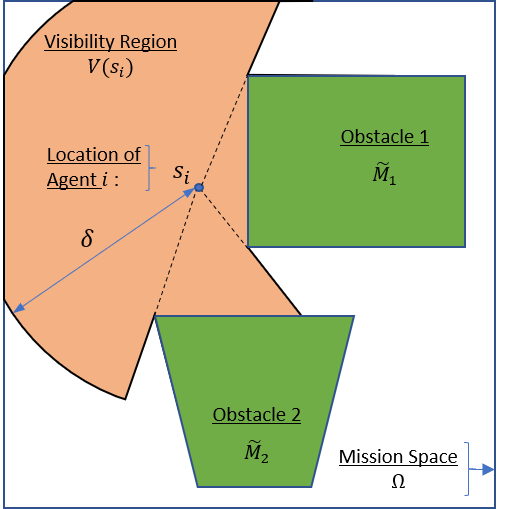
\includegraphics[width=2in]{Figures/Geometry.png}
    \caption{A mission space with one agent.}
    \label{Fig:Geometry}
\end{figure}


 
 
Assuming independently detecting agents, the probability of detecting an event occurring at $x \in F$ by at least one agent (when in an agent placement $\textbf{s}$) is given by $P(x,\textbf{s}) = 1-\prod_{i=1}^N \left[ 1-p(x,s_i) \right]$. This is more commonly known as the \emph{joint detection probability function}. Using the event density function and the joint detection probability function, the objective function of the multi-agent coverage problem can be written as
$H(\textbf{s}) = \int_\Omega R(x)P(x,\textbf{s})dx$. Therefore, the multi-agent coverage problem can be stated as
\begin{equation}\label{Eq:CoverageProblem}
    \textbf{s}^* = \underset{\textbf{s}:\, s_i \in F, \forall i\in [1,N]}{\arg\max}\ H(\textbf{s}).
\end{equation}


\subsection{Set function approach for multi-agent coverage problems}

To model the multi-agent coverage problem in \eqref{Eq:CoverageProblem} as a set function maximization problem of the form \eqref{Eq:SubmodularMaximizationProblem}, we use the following set of steps. First, the ground set $X=\{x_1,x_2,\ldots,x_M\}$ is created by discretizing the continuous feasible space $F \subset \R^2$. Next, a set variable is defined as $S = \{s_1,s_2,\ldots,s_N\}$ to represent the selected agent locations from the ground set $X$. Since we are interested in deploying only $N$ agents, a uniform matroid constraint of rank $N$ can be introduced as $S\in\mathcal{I}^N$ where $\mathcal{I}^N = \{Y:Y \subseteq X, \vert Y \vert \leq N\}$. Now the corresponding set function maximization problem for \eqref{Eq:CoverageProblem} can be written as 
\begin{equation}\label{Eq:SetCoverageMaximization}
    S^* = \underset{S\in\mathcal{I}^N}{\arg\max}\ H(S),
\end{equation}
where $H(S)$ (called the \emph{set coverage function}) is the set function version of the coverage objective function $H(\textbf{s})$, i.e., 
\begin{equation}\label{Eq:SetCoverageFunction}
    H(S) = \int_F R(x)(1-\prod_{s_i \in S} \left[1-p(x,s_i)\right])dx.
\end{equation}
The work in \cite{Sun2019} has established that $H(S)$ in \eqref{Eq:SetCoverageFunction} is a polymatroid set function. Hence, it is clear that the multi-agent coverage problem in \eqref{Eq:CoverageProblem} is a submodular maximization problem of the form \eqref{Eq:SubmodularMaximizationProblem}. 

As a consequence, we now can solve the multi-agent coverage problem conveniently using the greedy algorithm (Alg. \ref{Alg:GreedyAlgorithm}) and also get a performance bound that characterizes how close the obtained greedy coverage level is to the global optimal coverage level. As mentioned in Remark \ref{Rm:Improvements}, similar to the works in \cite{Sun2019,Sun2020}, a subsequent gradient ascent stage or an interchange stage can be added to further improve any greedy solution obtained for \eqref{Eq:SetCoverageMaximization}. However, as shown in Prop. \ref{Prop:Improvement}, such an improvement will only scale any performance bound (already found for the greedy solution) by a fixed constant factor. Therefore, in this paper, we omit executing such improvement stages and directly study the performance bounds found for the greedy solution. 



\subsection{Numerical Results}

The greedy algorithm (Alg. \ref{Alg:GreedyAlgorithm}), the newly proposed performance bound $\beta_u$ \eqref{Eq:Th:MainTheorem} ($\alpha_u$ in \eqref{Eq:Th:MainTheorem} was determined using \eqref{Eq:ExtGreedyCurvatureMeasure} with $Q=\bar{Q}$) and the existing other performance bounds: $\beta_f$ \eqref{Eq:FundamentalPerformanceBound}, $\beta_t$ \eqref{Eq:TotalCurvatureBoundTheory}, $\beta_g$ \eqref{Eq:GreedyCurvatureBoundTheory}, $\beta_e$ \eqref{Eq:ElementalCurvatureBoundTheory} and $\beta_p$ \eqref{Eq:PartialCurvatureBoundTheory} were all implemented for the considered class of multi-agent coverage problems in an interactive JavaScript-based simulator which is available at \url{http://www.bu.edu/codes/simulations/shiran27/CoverageFinal/} (the source code is available at: \url{https://github.com/shiran27/CoverageControl}). It may be used by the reader to reproduce the reported results and also to try different new problem configurations.   


In particular, mission spaces with three different obstacle arrangements named `General,' `Maze' and `Blank' were considered (can be seen in Fig. \ref{Fig:GeneralConfigBetaVsRange}(b), Fig. \ref{Fig:MazeConfigBetaVsN}(d) and Fig. \ref{Fig:BlankConfigBetaVsDecay}(b), respectively). In such mission space diagrams, obstacles are shown as dark green-colored blocks and agent locations are shown as red-colored dots. Moreover, light-colored areas indicate low coverage levels while dark-colored areas indicate the opposite.




\begin{figure}[!b]
    \centering
    \begin{subfigure}[t]{\columnwidth}
        \centering
        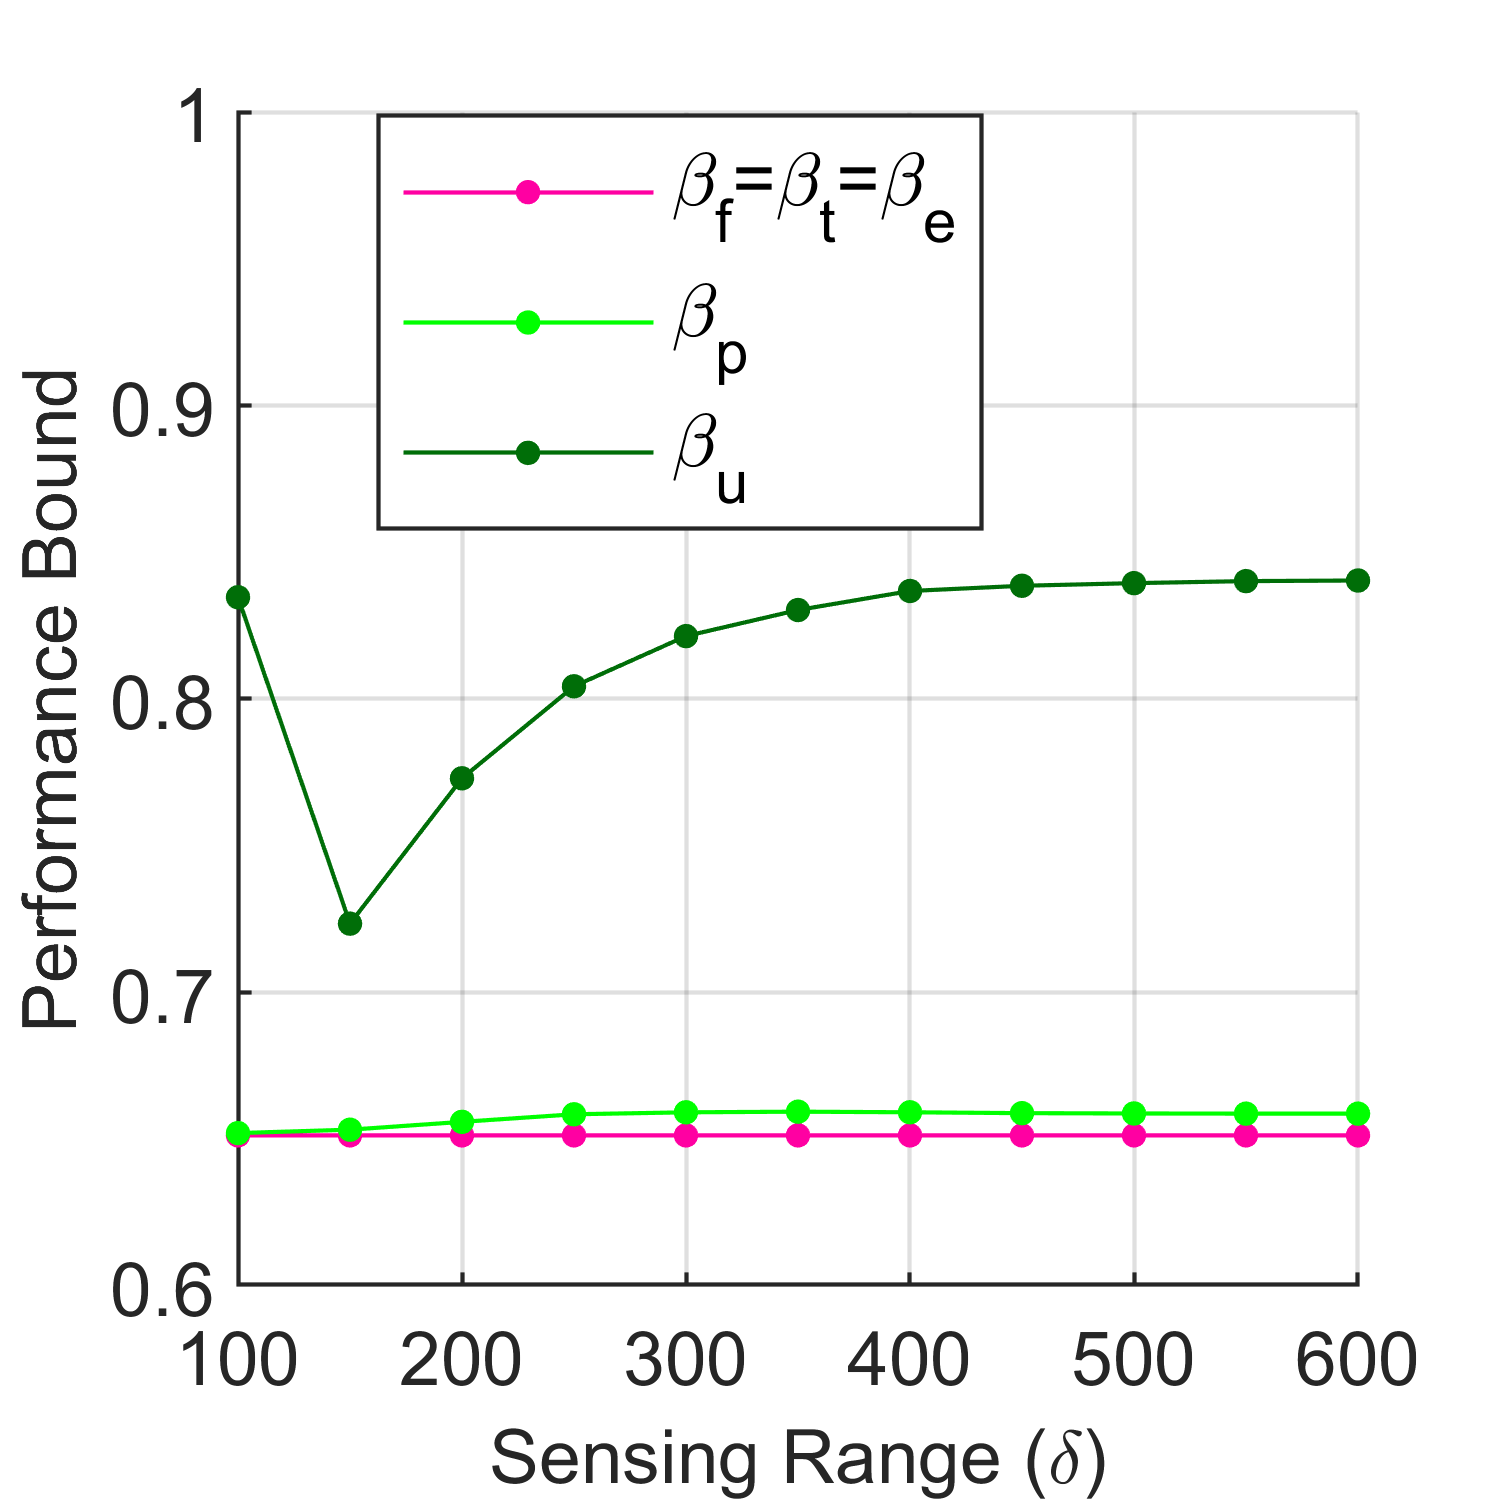
\includegraphics[width=2in]{Figures/Gen1.png}
        \caption{$\lambda=0.006, N=10$ \\ Average Improvement = $0.1591$}
    \end{subfigure}%
    \\
    \centering
    \begin{subfigure}[t]{0.105\textwidth}
        \centering
        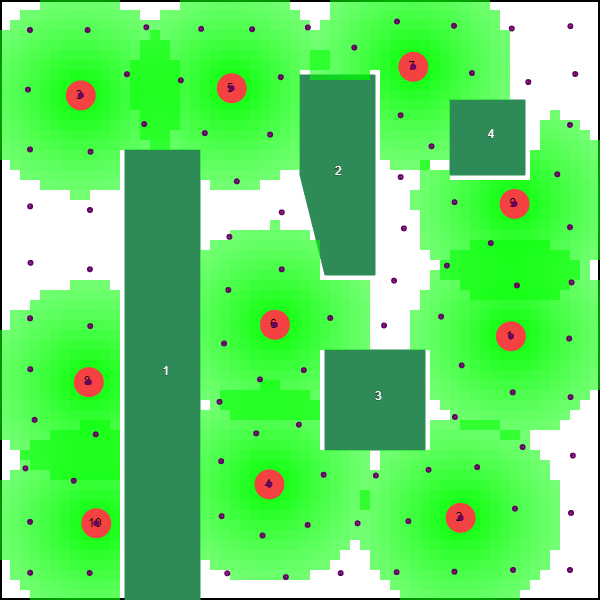
\includegraphics[width=\textwidth]{Figures/Gen1_1.png}
        \caption{$\delta=100$}
    \end{subfigure}\hspace{3mm}
    \begin{subfigure}[t]{0.105\textwidth}
        \centering
        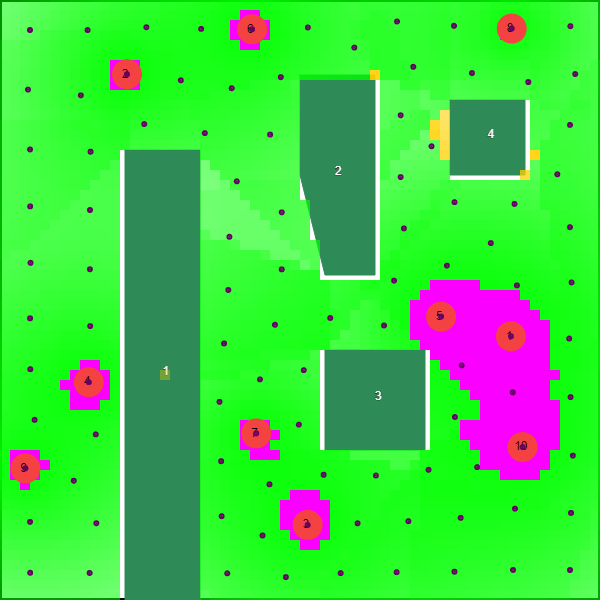
\includegraphics[width=\textwidth]{Figures/Gen1_2.png}
        \caption{$\delta=350$}
    \end{subfigure}\hspace{3mm}
    \begin{subfigure}[t]{0.105\textwidth}
        \centering
        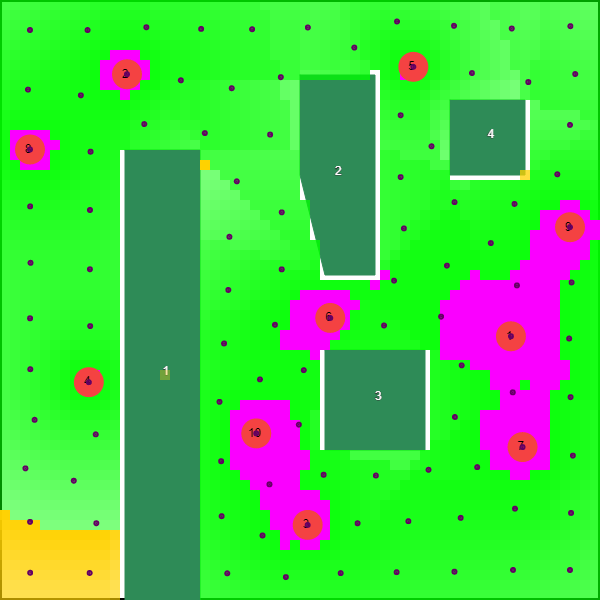
\includegraphics[width=\textwidth]{Figures/Gen1_3.png}
        \caption{$\delta=600$}
    \end{subfigure}
    \caption{Performance Bound vs. Sensing Range ($\delta$) for the General mission space configuration. Sub-figures (b)-(d) show three greedy solutions obtained for three different $\delta$ values.}
    \label{Fig:GeneralConfigBetaVsRange}
    % \vspace{-5mm}
\end{figure}



\begin{figure}[!b]
    \centering
    \begin{subfigure}[t]{\columnwidth}
        \centering
        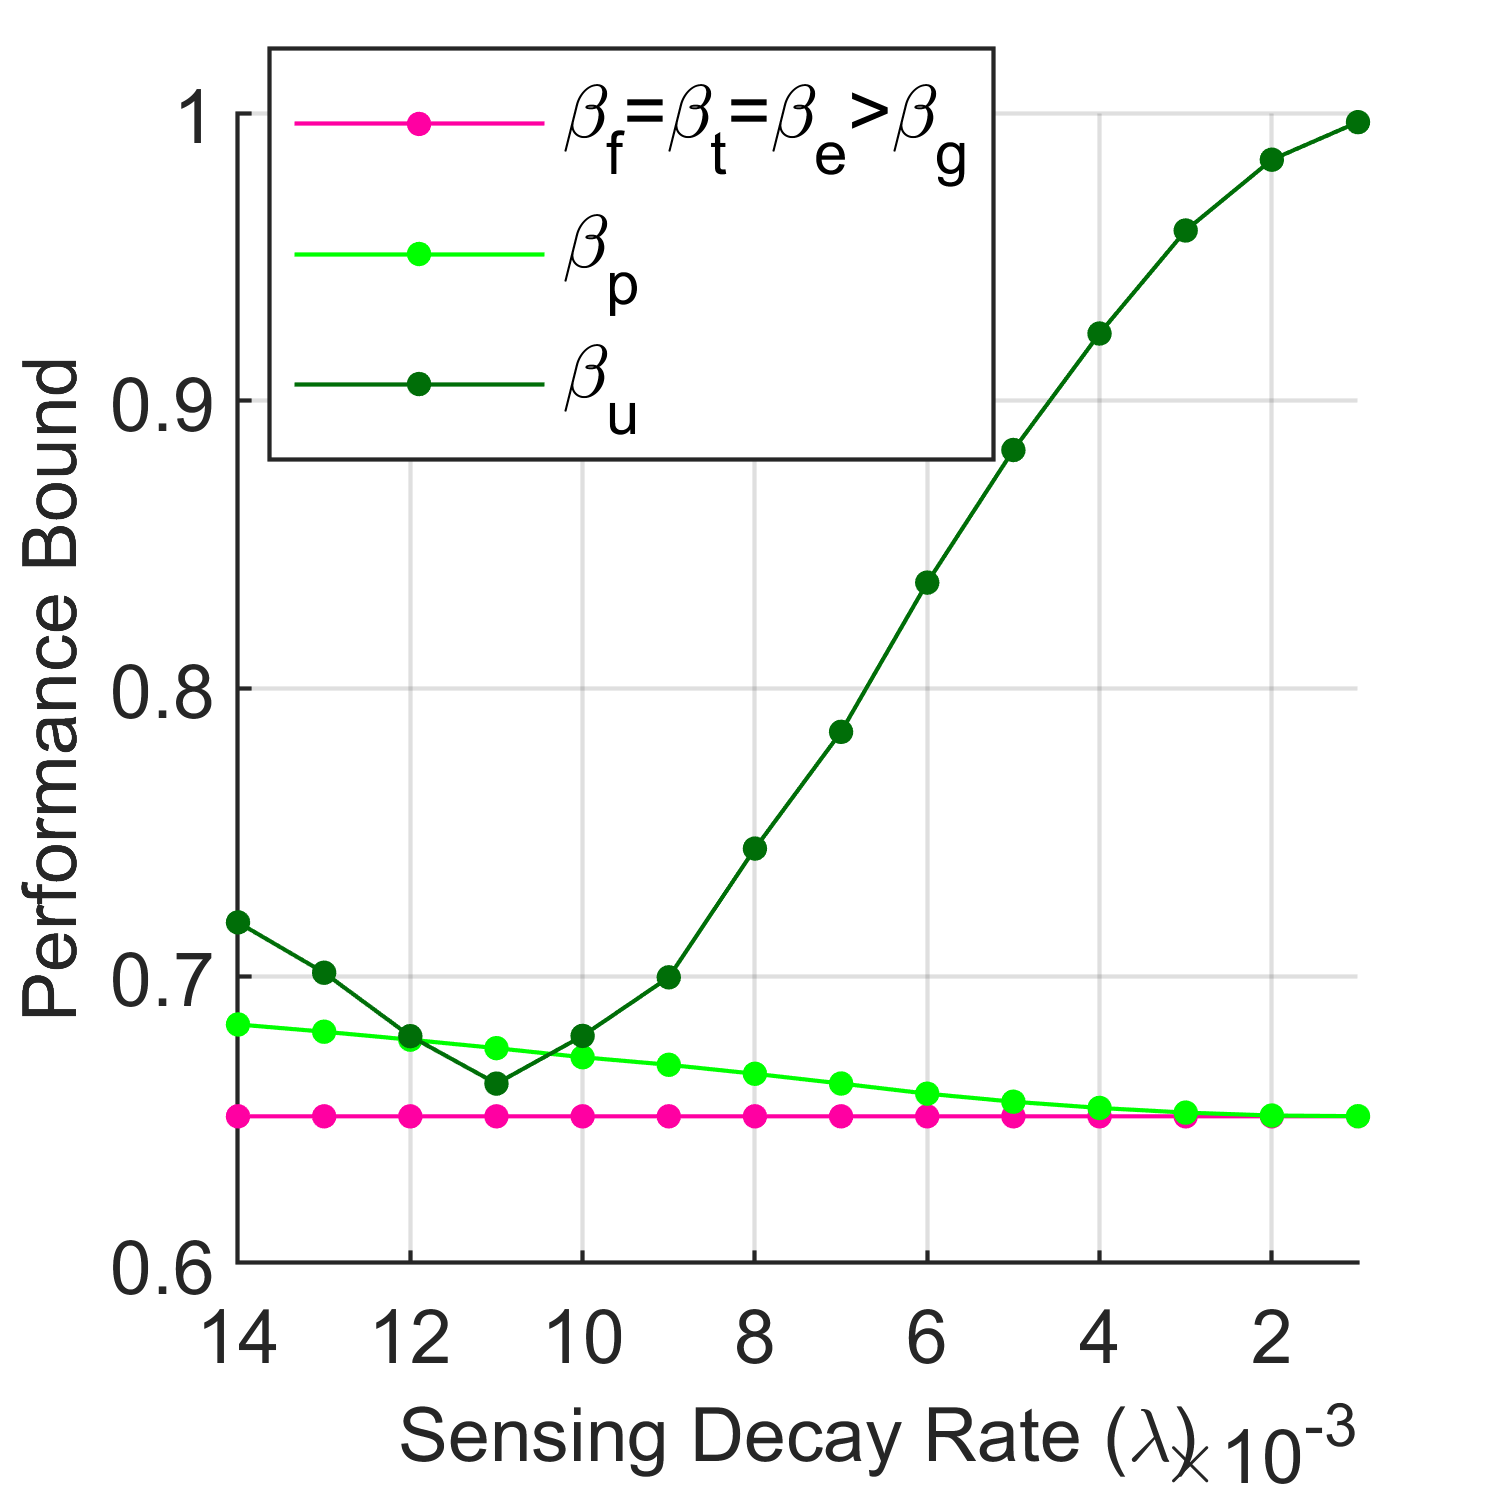
\includegraphics[width=2in]{Figures/Gen2.png}
        \caption{$\delta=400, N=10$ \\ Average Improvement = $0.1386$}
    \end{subfigure}%
    \\
    \centering
    \begin{subfigure}[t]{0.105\textwidth}
        \centering
        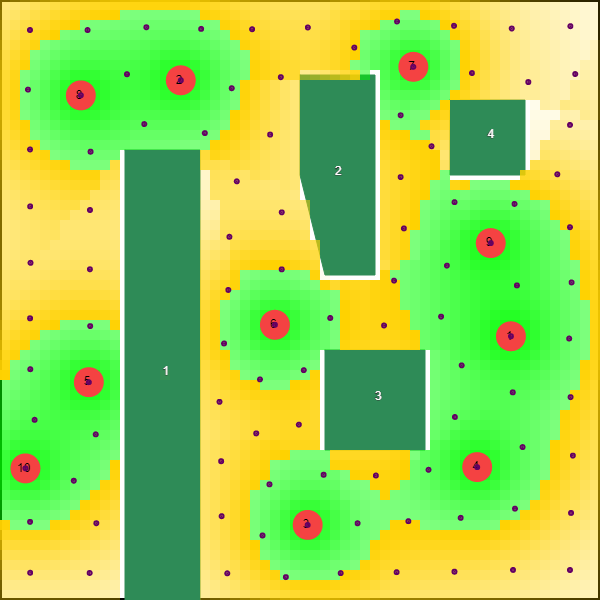
\includegraphics[width=\textwidth]{Figures/Gen2_1.png}
        \caption{$\lambda=0.014$}
    \end{subfigure}\hspace{3mm}
    \begin{subfigure}[t]{0.105\textwidth}
        \centering
        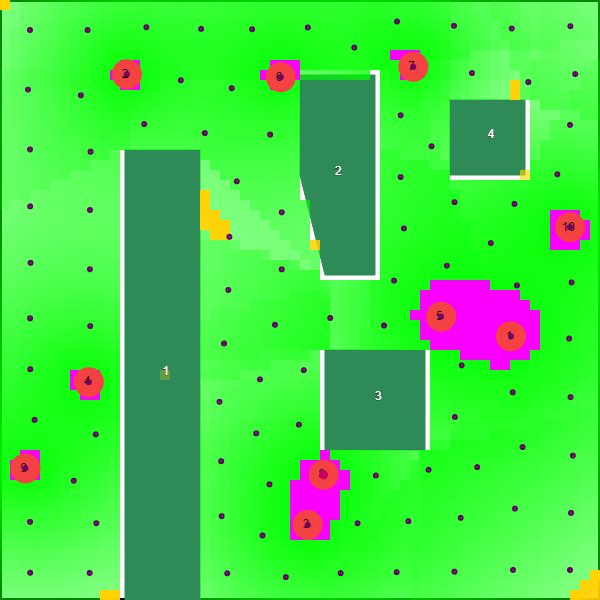
\includegraphics[width=\textwidth]{Figures/Gen2_2.png}
        \caption{$\lambda=0.007$}
    \end{subfigure}\hspace{3mm}
    \begin{subfigure}[t]{0.105\textwidth}
        \centering
        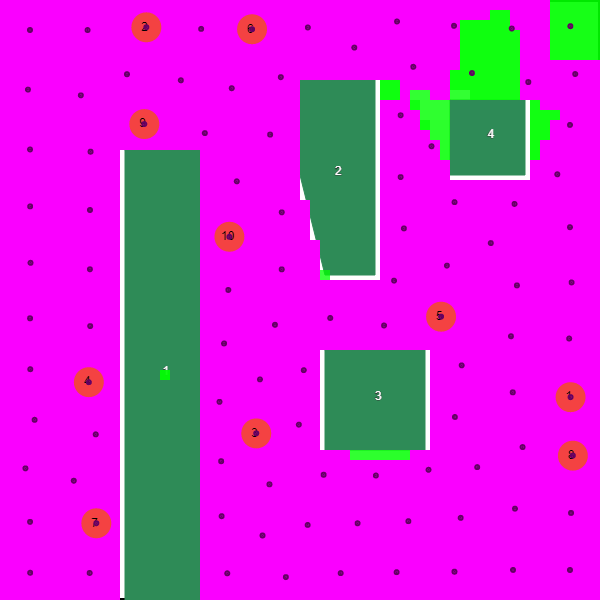
\includegraphics[width=\textwidth]{Figures/Gen2_3.png}
        \caption{$\lambda=0.001$}
    \end{subfigure}
    \caption{Performance Bound vs. Sensing Decay Rate ($\lambda$) for the General mission space configuration. Sub-figures (b)-(d) show three greedy solutions obtained for three different $\lambda$ values.}
    \label{Fig:GeneralConfigBetaVsDecay}
    % \vspace{-5mm}
\end{figure}




\begin{figure*}[t]
    \centering
    \begin{subfigure}[t]{0.33\textwidth}
        \centering
        \captionsetup{justification=centering}
        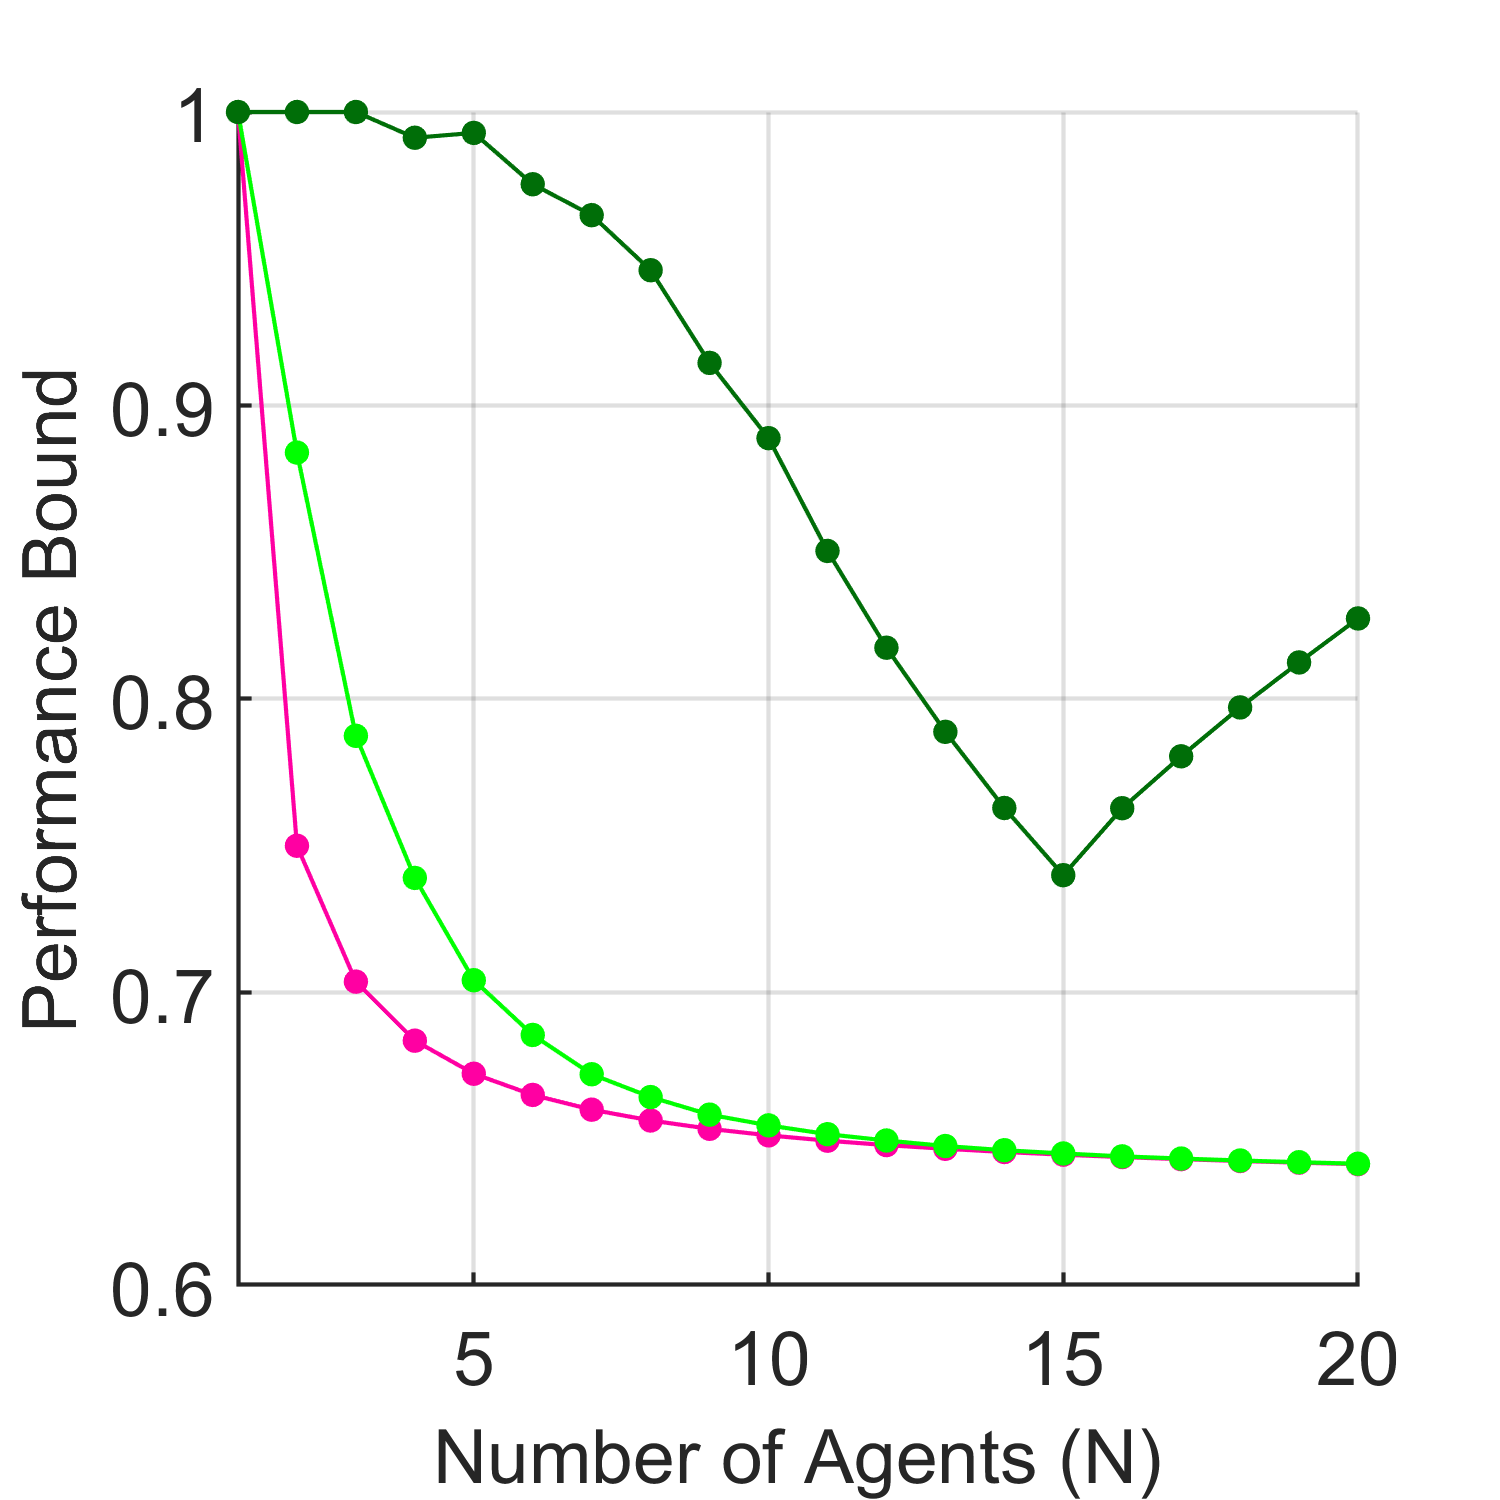
\includegraphics[width=2in]{Figures/Maze4.png}
        \caption{$\delta = 200, \lambda = 0.008$ \\ Average Improvement = $0.1855$}
    \end{subfigure}%
    \hfill
    \begin{subfigure}[t]{0.33\textwidth}
        \centering
        \captionsetup{justification=centering}
        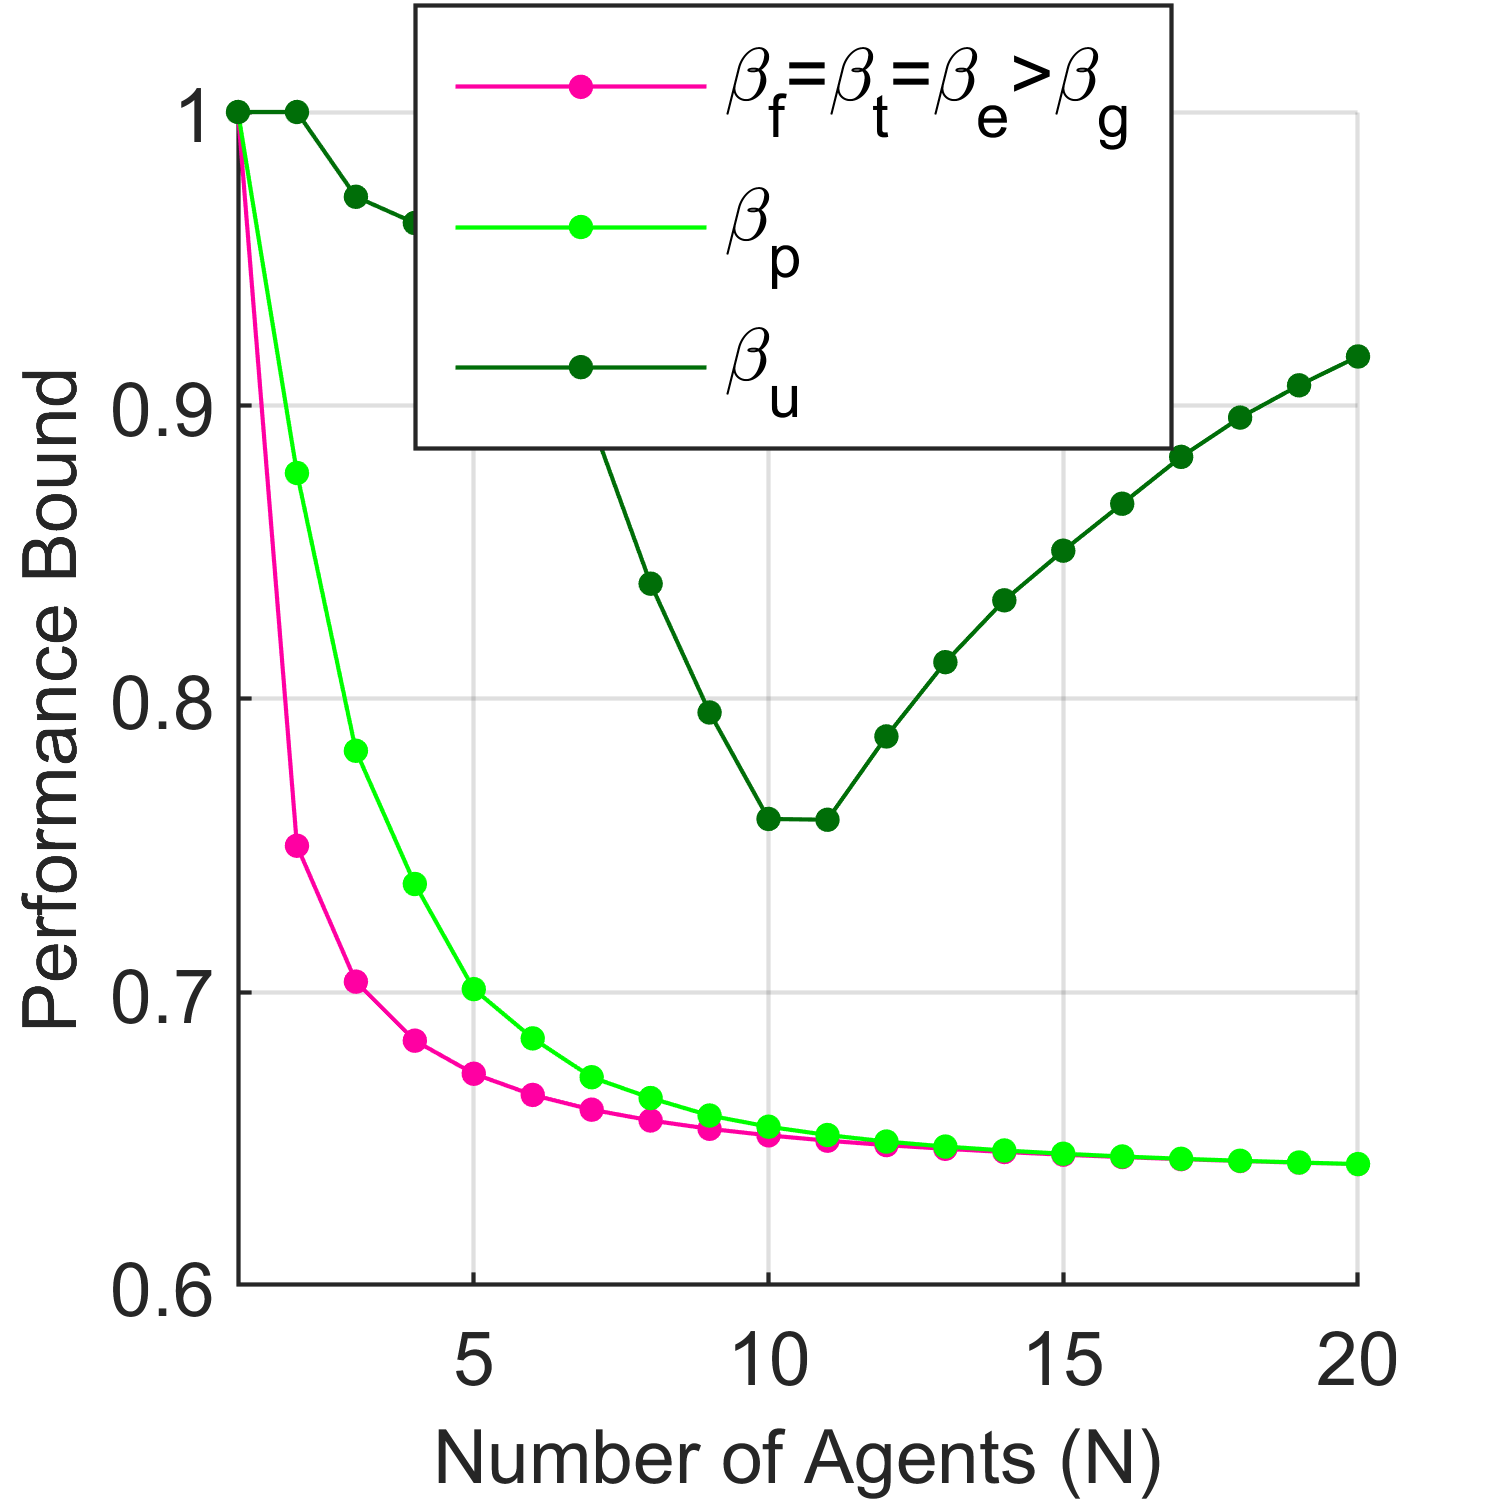
\includegraphics[width=2in]{Figures/Maze1.png}
        \caption{$\delta = 300, \lambda = 0.006$ \\ Average Improvement = $0.1856$}
    \end{subfigure}
    \hfill
    \begin{subfigure}[t]{0.33\textwidth}
        \centering
        \captionsetup{justification=centering}
        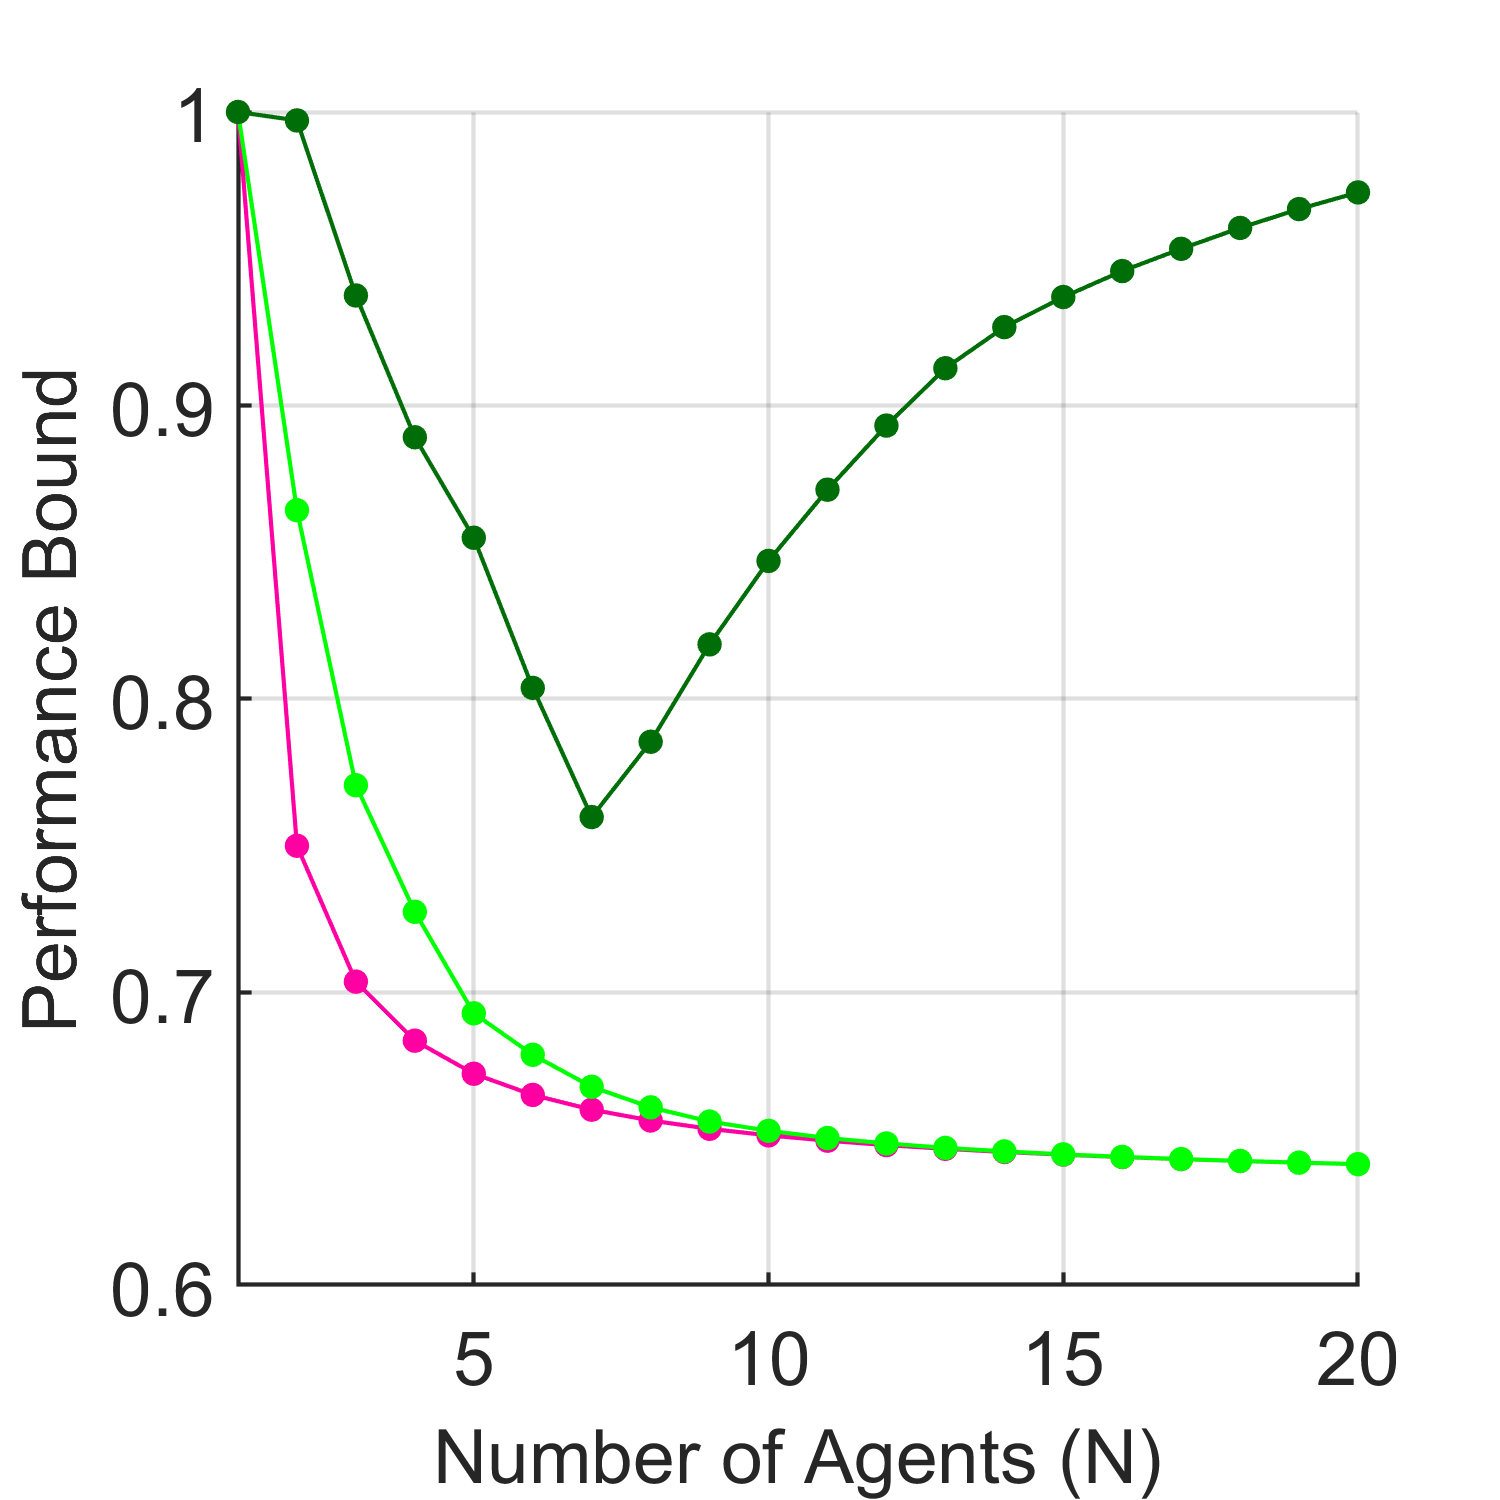
\includegraphics[width=2in]{Figures/Maze2.png}
        \caption{$\delta = 400, \lambda = 0.004$ \\ Average Improvement = $0.2106$}
    \end{subfigure}
    \\
    \centering
    \begin{subfigure}[t]{0.1\textwidth}
        \centering
        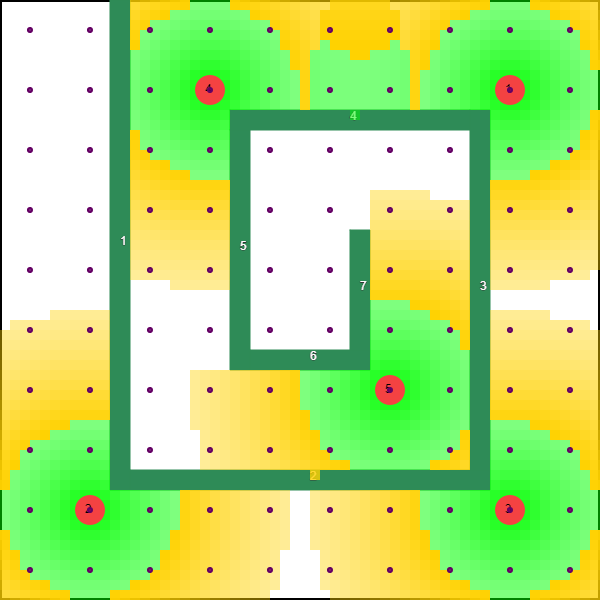
\includegraphics[width=\textwidth]{Figures/Maze4_1.png}
        \caption{$N=5$}
    \end{subfigure}\hfill
    \begin{subfigure}[t]{0.1\textwidth}
        \centering
        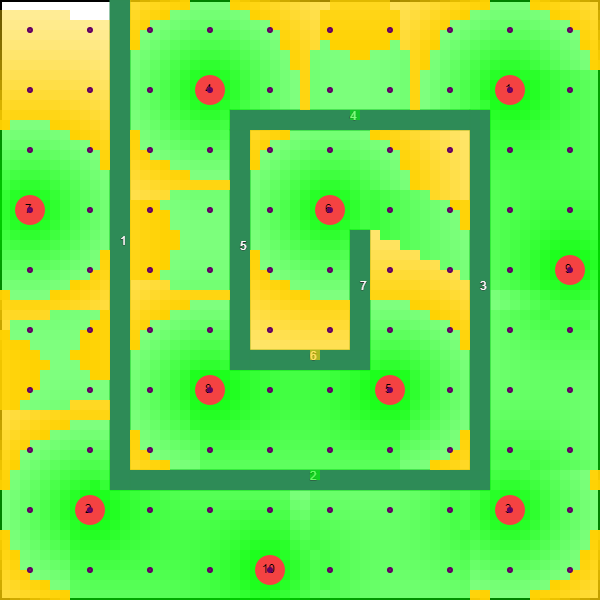
\includegraphics[width=\textwidth]{Figures/Maze4_2.png}
        \caption{$N=10$}
    \end{subfigure}\hfill
    \begin{subfigure}[t]{0.1\textwidth}
        \centering
        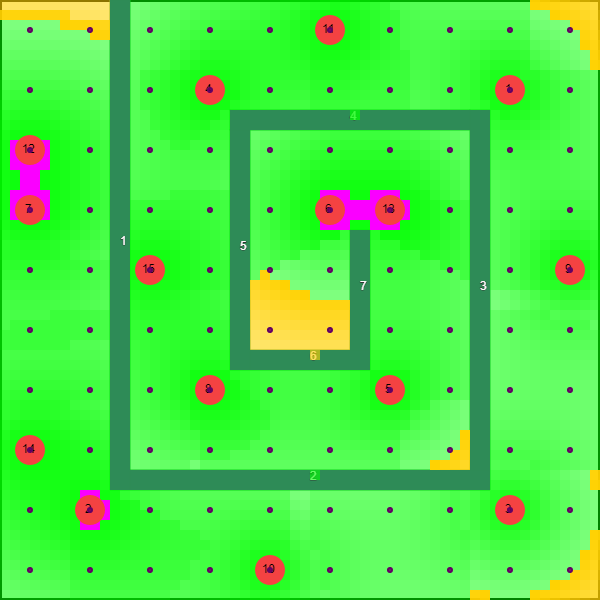
\includegraphics[width=\textwidth]{Figures/Maze4_3.png}
        \caption{$N=15$}
    \end{subfigure}
    \hspace{5mm}
    \begin{subfigure}[t]{0.1\textwidth}
        \centering
        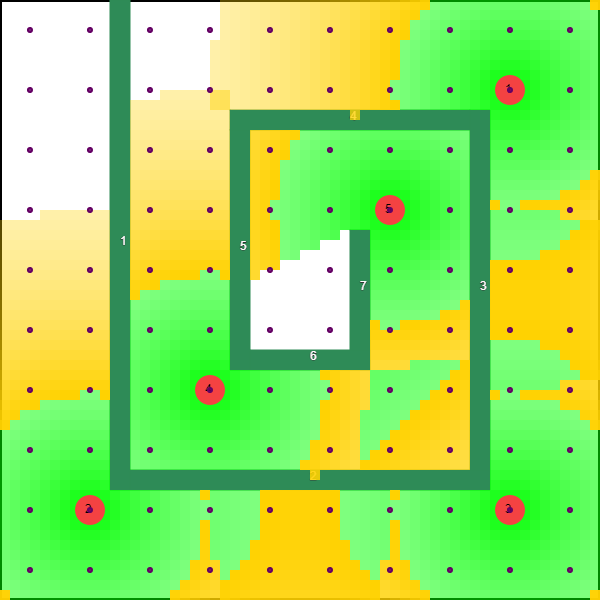
\includegraphics[width=\textwidth]{Figures/Maze1_1.png}
        \caption{$N=5$}
    \end{subfigure}
    \hfill
    \begin{subfigure}[t]{0.1\textwidth}
        \centering
        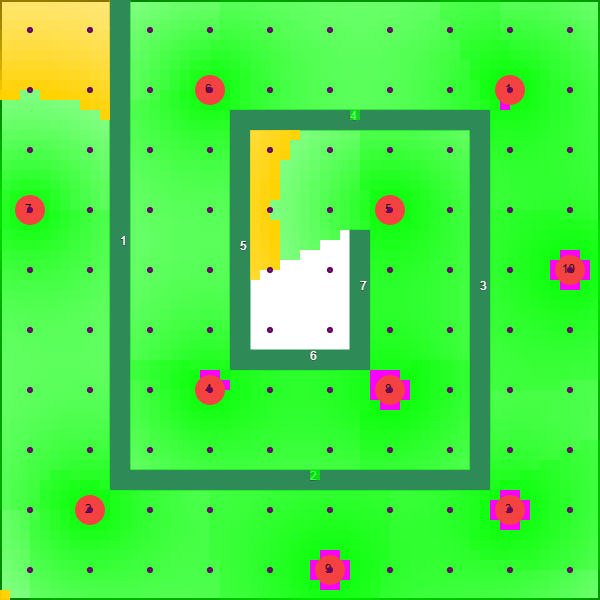
\includegraphics[width=\textwidth]{Figures/Maze1_2.png}
        \caption{$N=10$}
    \end{subfigure}
    \hfill
    \begin{subfigure}[t]{0.1\textwidth}
        \centering
        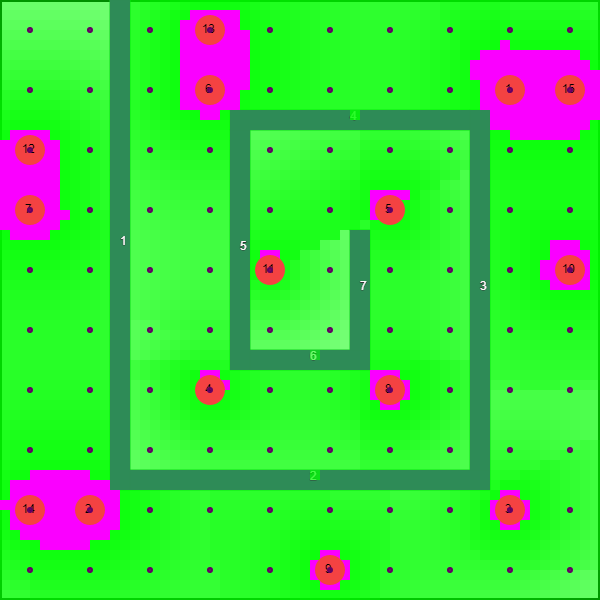
\includegraphics[width=\textwidth]{Figures/Maze1_3.png}
        \caption{$N=15$}
    \end{subfigure}
    \hspace{5mm}
    \begin{subfigure}[t]{0.1\textwidth}
        \centering
        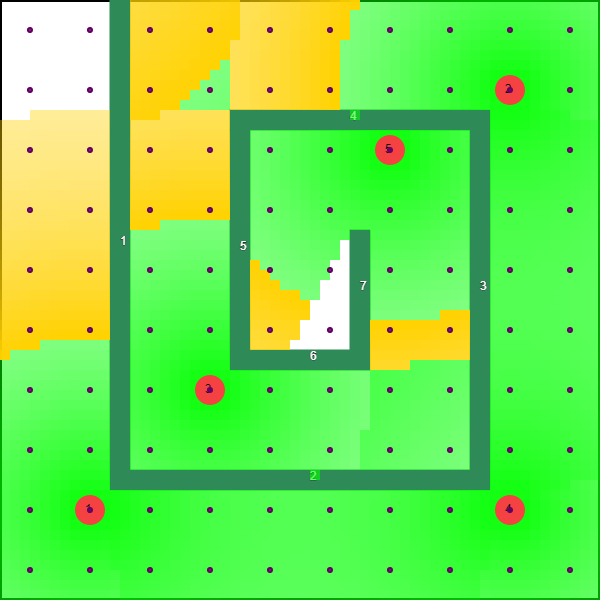
\includegraphics[width=\textwidth]{Figures/Maze2_1.png}
        \caption{$N=5$}
    \end{subfigure}
    \hfill
    \begin{subfigure}[t]{0.1\textwidth}
        \centering
        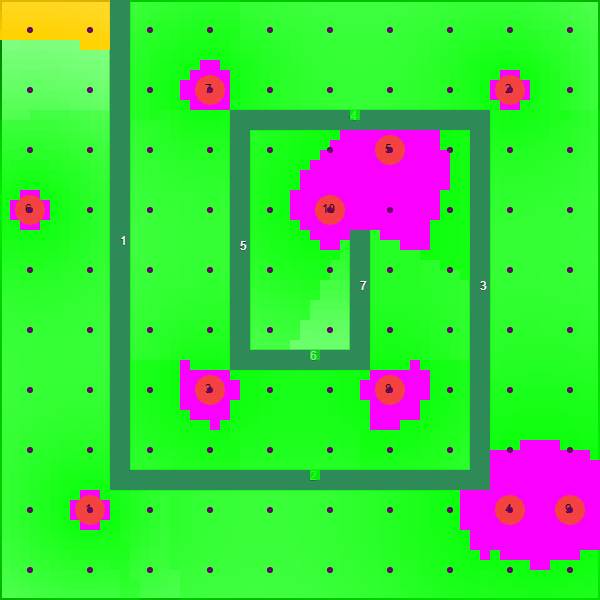
\includegraphics[width=\textwidth]{Figures/Maze2_2.png}
        \caption{$N=10$}
    \end{subfigure}
    \hfill
    \begin{subfigure}[t]{0.1\textwidth}
        \centering
        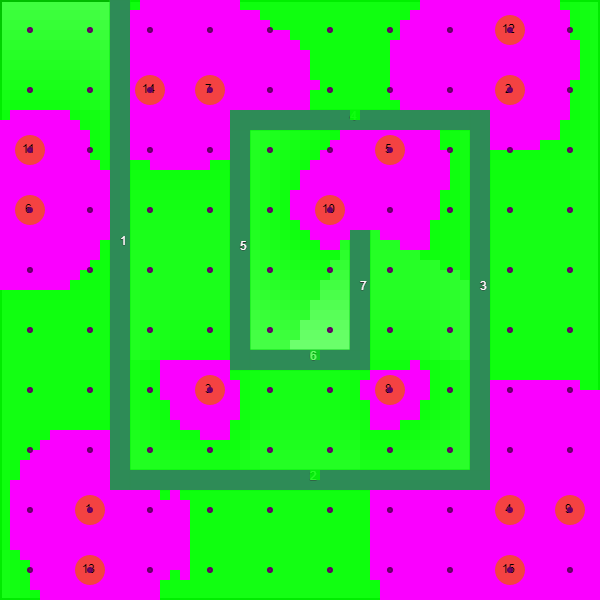
\includegraphics[width=\textwidth]{Figures/Maze2_3.png}
        % \caption{$N=15$}
    \end{subfigure}
    \caption{Performance Bound Vs Number of Agents ($N$) for the Maze mission space configuration: Agent sensing capabilities (or proportionately, the strength of the submodularity property of the set coverage objective) is: (a) weak, (b) moderate and (c) strong. Each of the corresponding three sub-figure groups (d)-(f), (g)-(i) and (j)-(l) shows three greedy solutions obtained for different $N$ values.}
    \label{Fig:MazeConfigBetaVsN}
\end{figure*}





\begin{figure}[!h]
    \centering
    \begin{subfigure}[t]{\columnwidth}
        \centering
        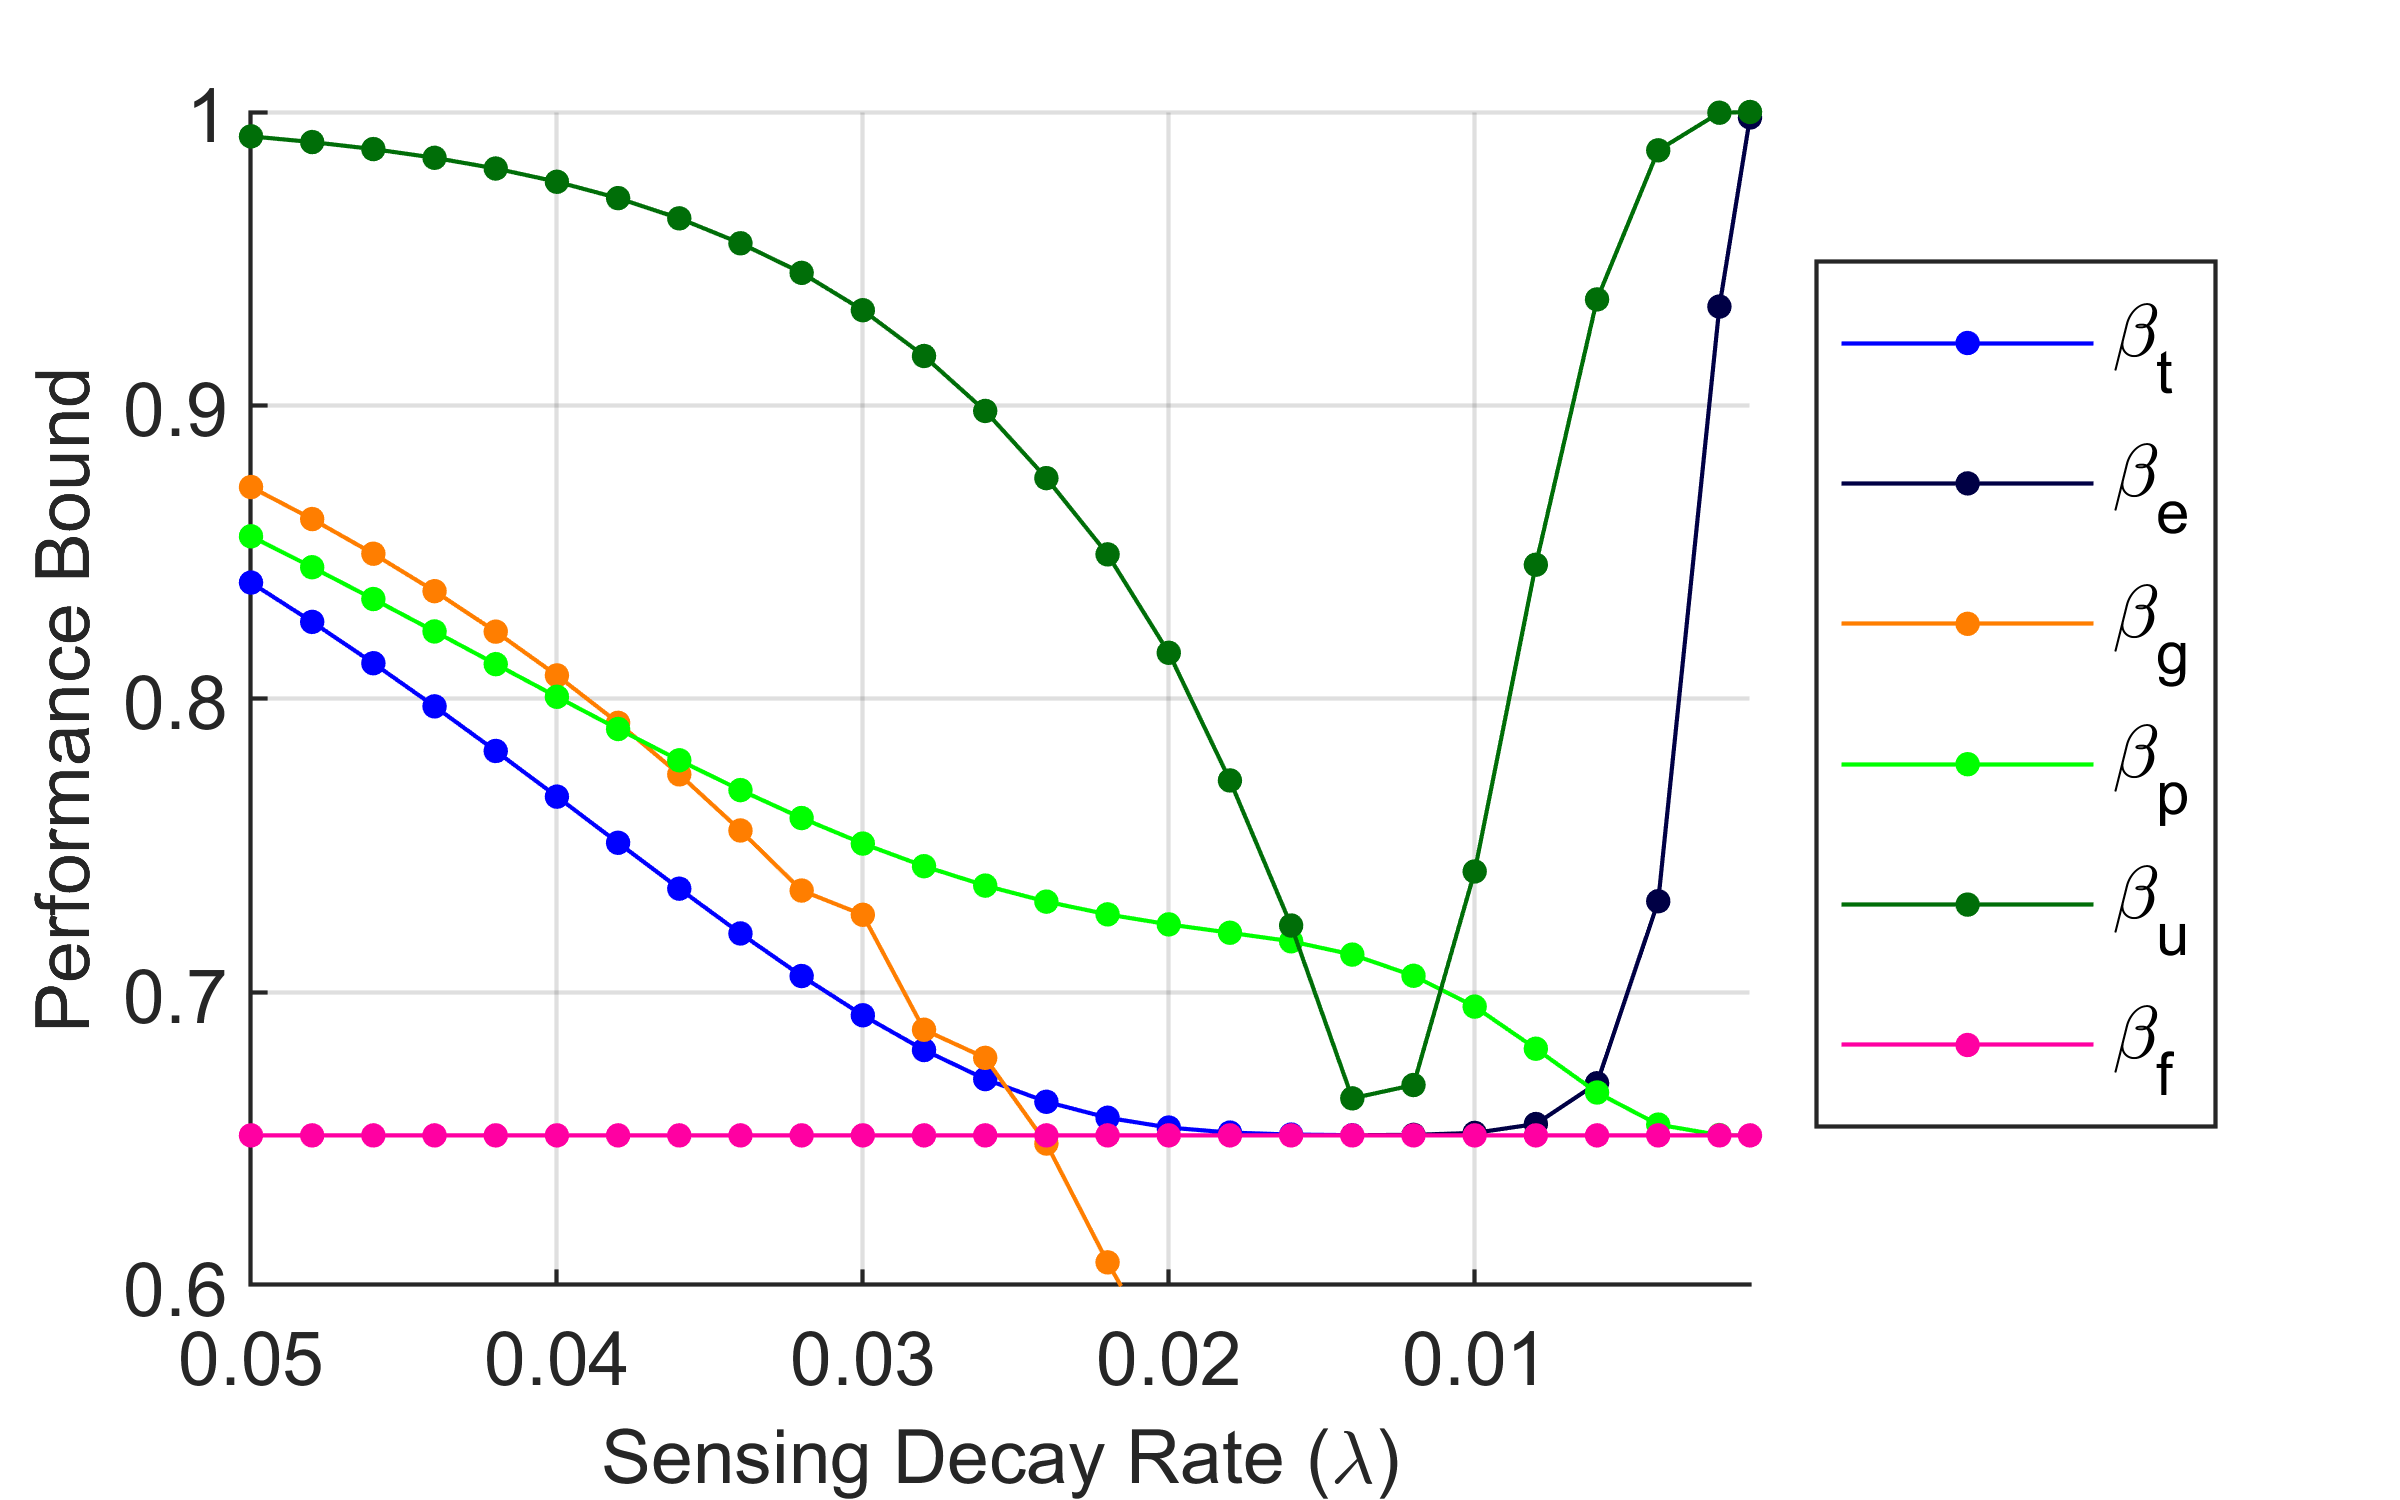
\includegraphics[width=3.2in]{Figures/Blank2.png}
        \caption{$\delta=800, N=10$ \\ Average Improvement = $0.1248$}
    \end{subfigure}%
    \\
    \centering
    \begin{subfigure}[t]{0.105\textwidth}
        \centering
        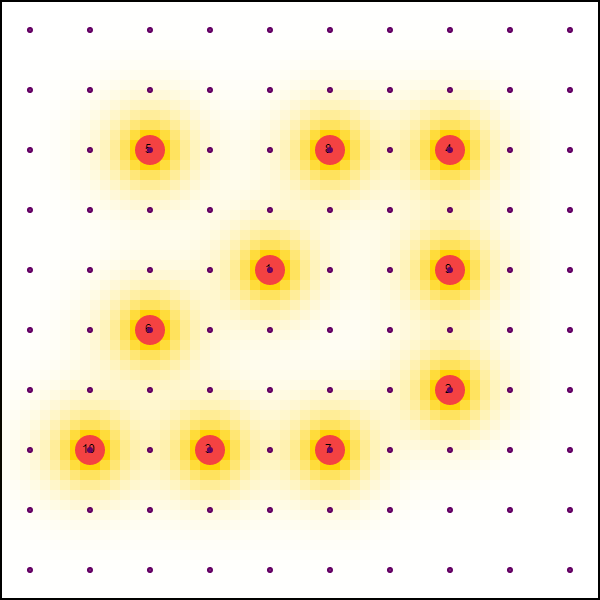
\includegraphics[width=\textwidth]{Figures/Blank2_1.png}
        \caption{$\lambda=0.046$}
    \end{subfigure}\hspace{3mm}
    \begin{subfigure}[t]{0.105\textwidth}
        \centering
        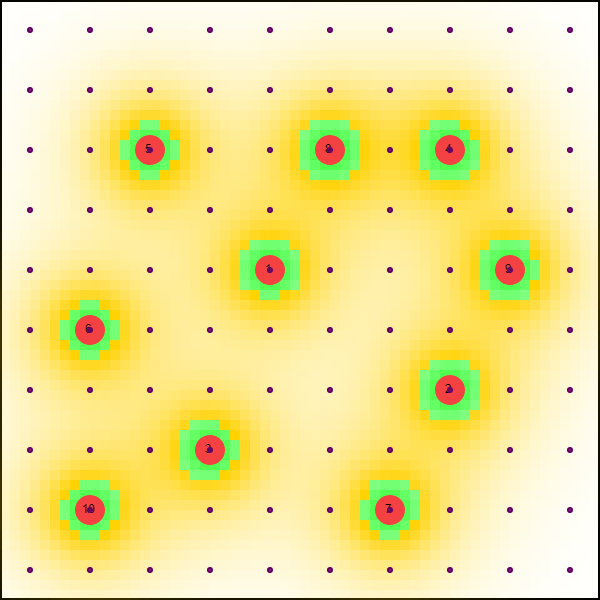
\includegraphics[width=\textwidth]{Figures/Blank2_2.png}
        \caption{$\lambda=0.026$}
    \end{subfigure}\hspace{3mm}
    \begin{subfigure}[t]{0.105\textwidth}
        \centering
        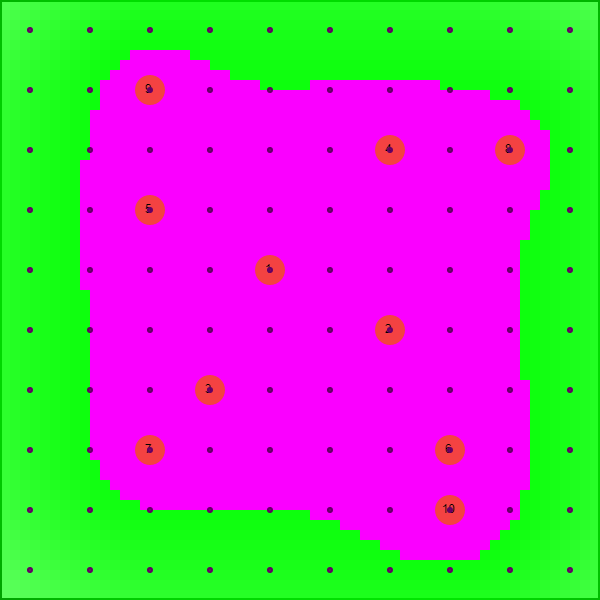
\includegraphics[width=\textwidth]{Figures/Blank2_3.png}
        \caption{$\lambda=0.006$}
    \end{subfigure}
    \caption{Performance Bound vs. Sensing Decay Rate ($\lambda$) for the Blank mission space configuration. Sub-figures (b)-(d) show three greedy solutions obtained for three different $\lambda$ values.}
    \label{Fig:BlankConfigBetaVsDecay}
\end{figure}



The main focus here is to study the behavior of different performance bounds (found for the greedy solution) under different coverage problem configurations. In each experiment shown in Figs. \ref{Fig:GeneralConfigBetaVsDecay}-\ref{Fig:BlankConfigBetaVsDecay}, one of the three parameters: (\romannum{1}) sensing range $\delta$, (\romannum{2}) sensing decay rate $\lambda$ or (\romannum{3}) the number of deployed agents $N$, was varied while keeping the other two fixed. Note that as $\delta$ increases or $\lambda$ decreases or $N$ increases, the \emph{agent sensing capability} over the mission space also increases. For convenience, each graph has been drawn so that along its $x$-axis, the agent sensing capability increases. It is easy to see that agent sensing capability directly maps to the strength of the submodularity property of the set coverage objective function (i.e., agents with high sensing capabilities make the submodularity property of the corresponding set coverage objective function strong, and vice versa). 
In the graphs shown in Figs. \ref{Fig:GeneralConfigBetaVsRange}(a), \ref{Fig:GeneralConfigBetaVsDecay}(a), \ref{Fig:MazeConfigBetaVsN}(a), \ref{Fig:MazeConfigBetaVsN}(b), \ref{Fig:MazeConfigBetaVsN}(c) and \ref{Fig:BlankConfigBetaVsDecay}(a), whenever only a few of the said performance bounds have been drawn, it means the other performance bounds were found redundant (no better than $\beta_f$). The \emph{average improvement} value reported in each such graph (caption) was computed by taking the average of $(\beta_u-\max\{\beta_f,\beta_t,\beta_g,\beta_e,\beta_f\})$ value across all the corresponding data points.



Across almost all the numerical results shown (see Fig. \ref{Fig:GeneralConfigBetaVsDecay}(a), $\lambda=11\times 10^{-3}$ case for an exception), the proposed extended greedy curvature based performance bound $\beta_u$ has shown the best performance bounds irrespective of the level of the agent sensing capabilities (i.e., irrespective of the strength of the submodularity property). In particular, the dip in the $\beta_u$ curve seen in each of the Figs. \ref{Fig:GeneralConfigBetaVsRange}, \ref{Fig:GeneralConfigBetaVsDecay}, \ref{Fig:MazeConfigBetaVsN}(a), \ref{Fig:MazeConfigBetaVsN}(b), \ref{Fig:MazeConfigBetaVsN}(c) and \ref{Fig:BlankConfigBetaVsDecay} point out that using a greedy algorithm to solve a multi-agent coverage problem is most challenging when the agents have a moderate sensing capability. Therefore, in such scenarios, the use of a greedy solution improvement scheme (see Remark \ref{Rm:Improvements}) can be recommended. We also highlight that in each $\beta_u$ curve, the decreasing set of data points (to the left of the dip point) have come from the extended greedy curvature measure $\alpha_u = \alpha^1_u$ (that can be computed in the very first greedy iteration). Hence, in all such scenarios, no extra greedy iterations were required. 


To further study this, let us denote $i^*$ as the argmin value of the problem \eqref{Eq:ExtGreedyCurvatureMeasure}. In other words, $i^*$ is the minimum number of greedy iterations required to obtain the extended greedy curvature measure $\alpha_u = \alpha^{i^*}_u$ \eqref{Eq:ExtGreedyCurvatureMeasure} and the corresponding performance bound $\beta_u=f(Y^G)/\alpha^{i^*}_u$ \eqref{Eq:Th:MainTheorem}. For the same experiments that generated the results shown in Figs. \ref{Fig:GeneralConfigBetaVsRange}(a) and \ref{Fig:GeneralConfigBetaVsDecay}(a), the corresponding $i^*$ vs $\beta_u$ behaviors observed (under different $\lambda$ and $\alpha$ values) are illustrated in Figs. \ref{Fig:GeneralConfigBetaVsRangeVsiStar} and  \ref{Fig:GeneralConfigBetaVsDecayVsiStar}, respectively. Note that the red curves in Figs. \ref{Fig:GeneralConfigBetaVsRangeVsiStar}(b) and  \ref{Fig:GeneralConfigBetaVsDecayVsiStar}(b) imply that the number of greedy iterations required to compute the proposed extended greedy curvature based performance bound $\beta_u$ \eqref{Eq:Th:MainTheorem} (i.e., $i^*$) is generally non-trivial and typically $N<i^*<M$.    
Note also that the same curves indicate the need for a higher number of greedy iterations to compute the proposed performance bound $\beta_u$ \eqref{Eq:Th:MainTheorem} (i.e., $i^*\gg N$) whenever the agents have a moderate sensing capability. This observation is in line with our previous conclusion that a multi-agent coverage problem is most challenging when the agents have a moderate sensing capability. 



\begin{figure}[!t]
    \centering
    \begin{subfigure}[t]{\columnwidth}
        \centering
        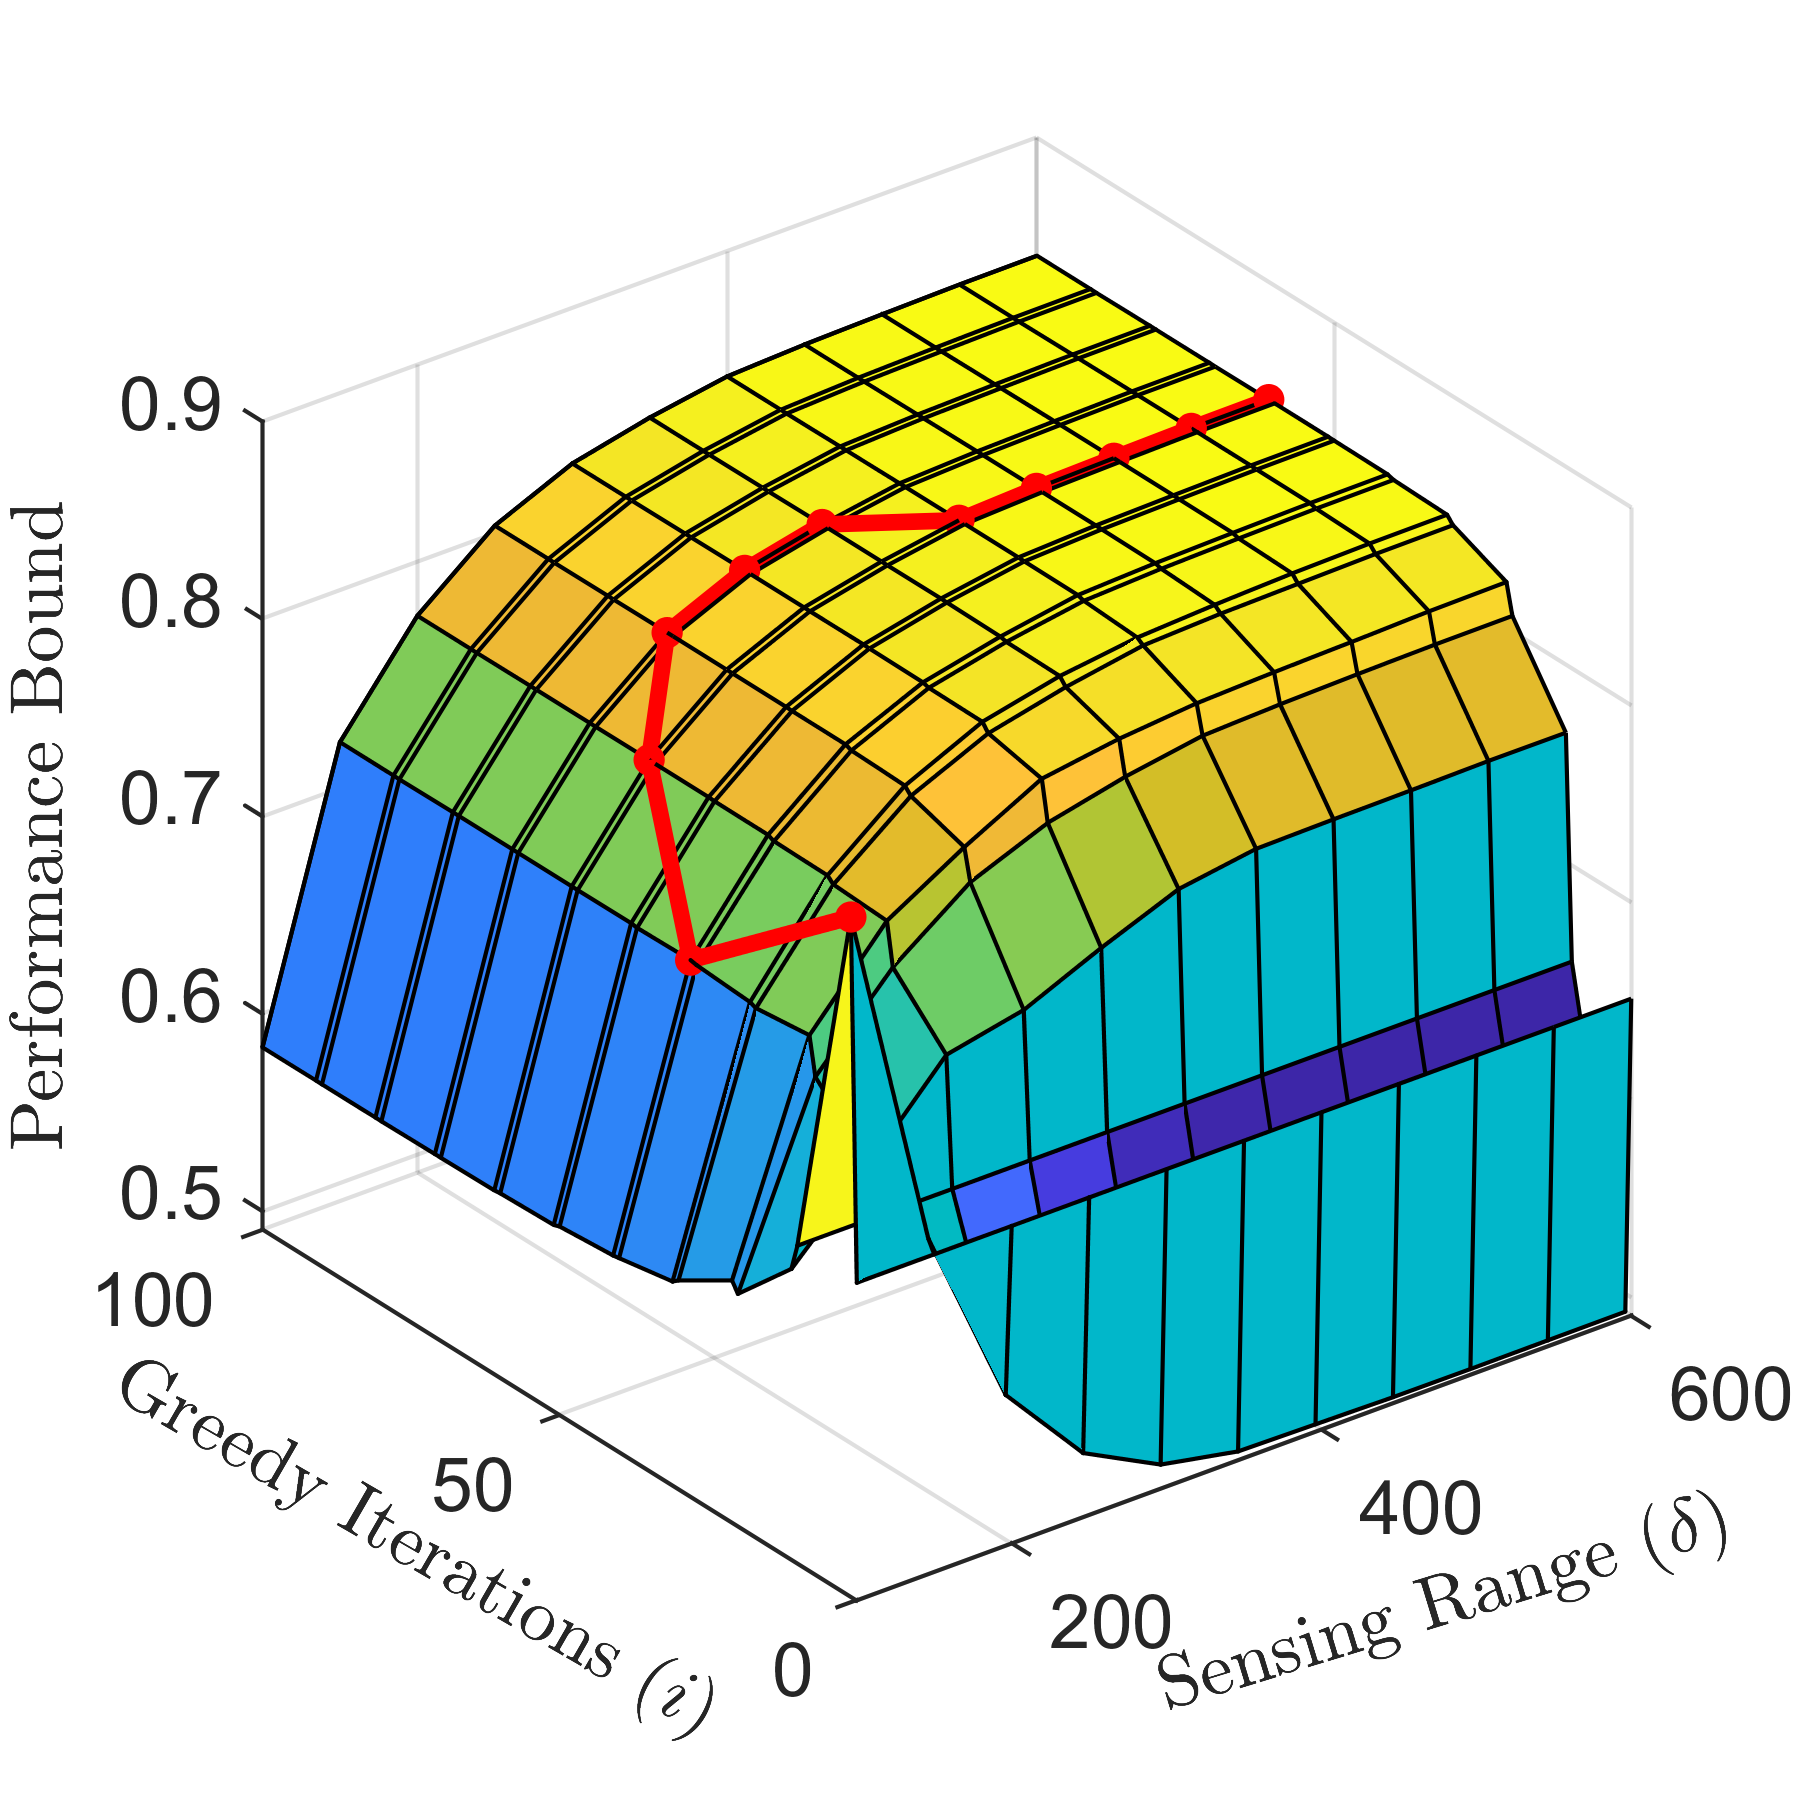
\includegraphics[width=2.5in]{Figures/Gen1_Exd.png}
        \caption{The surface plot. Red line: $\beta_u$ vs. $\delta$  vs. $i^*$.}
    \end{subfigure}%
    \\
    \centering
    \begin{subfigure}[t]{0.17\textwidth}
        \centering
        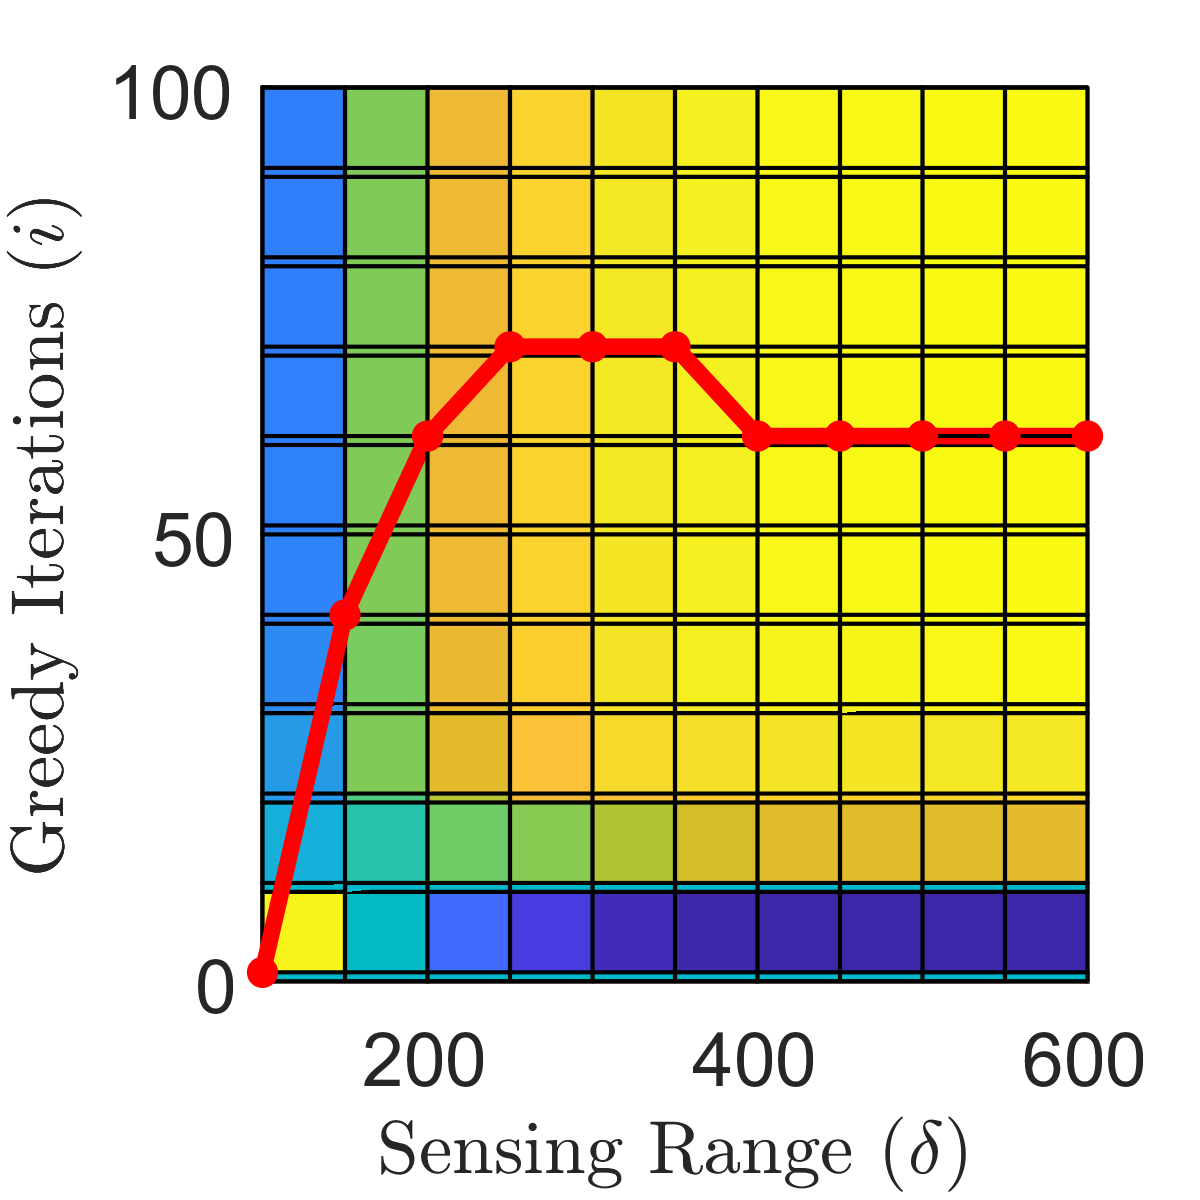
\includegraphics[width=\textwidth]{Figures/Gen1_Exd2.png}
        \caption{XY-View}
    \end{subfigure}
    \hspace{3mm}
    \begin{subfigure}[t]{0.17\textwidth}
        \centering
        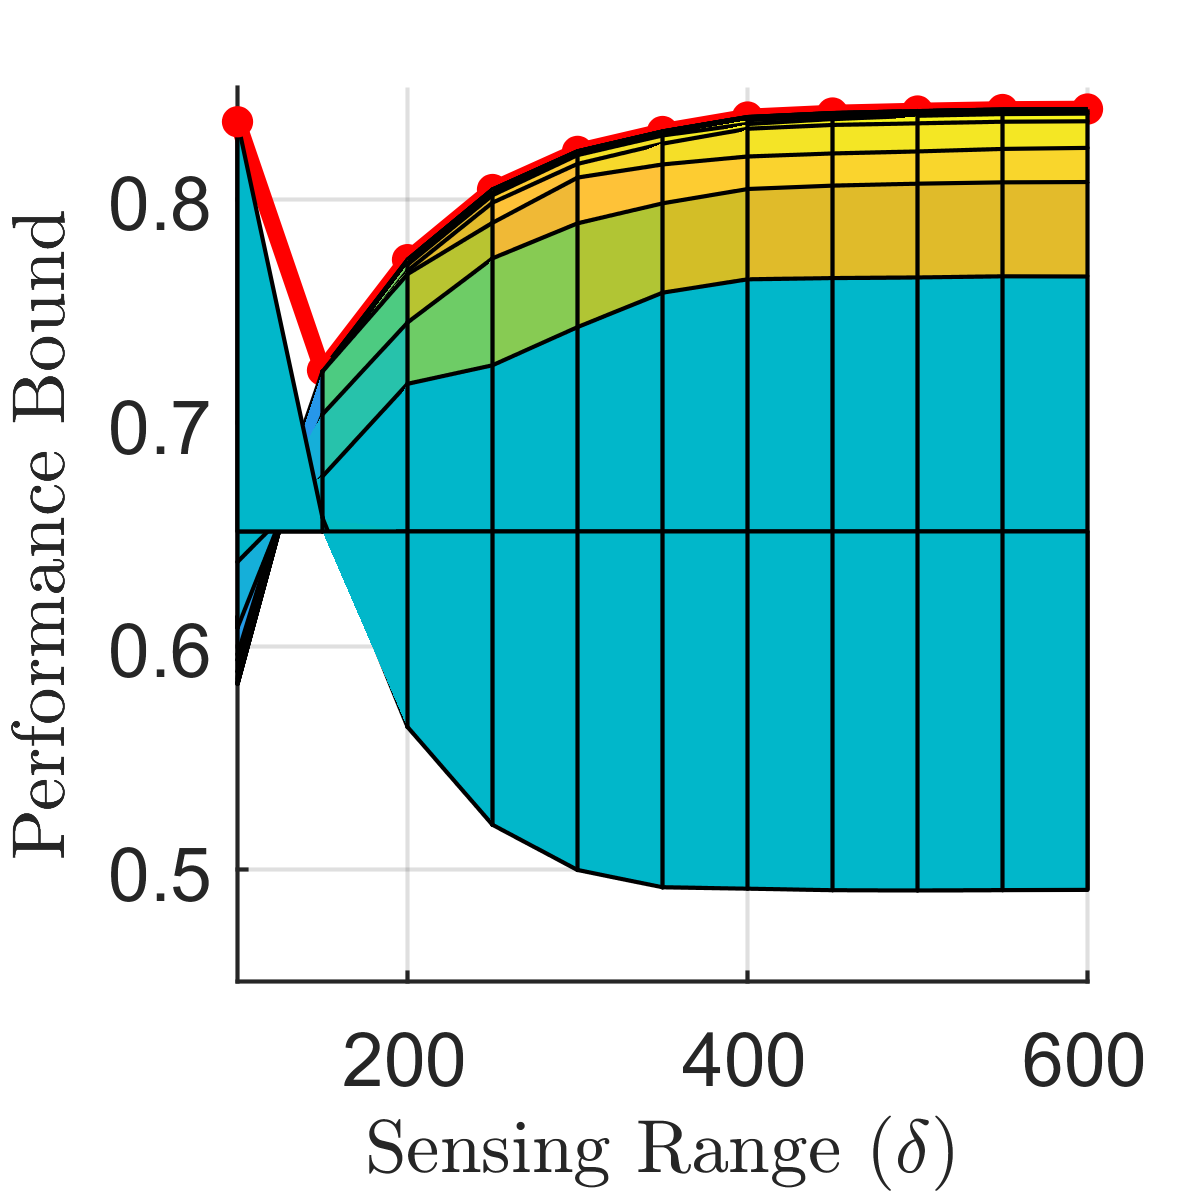
\includegraphics[width=\textwidth]{Figures/Gen1_Exd3.png}
        \caption{XZ-View (Fig. \ref{Fig:GeneralConfigBetaVsRange}(a))}
    \end{subfigure}
    \caption{Extend Greedy Curvature Based Performance Bound vs. Sensing Range ($\delta$) vs. No. of Greedy Iterations for the General mission space configuration with $\lambda=0.006$, $N=10$.}
    \label{Fig:GeneralConfigBetaVsRangeVsiStar}
\end{figure}



\begin{figure}[!t]
    \centering
    \begin{subfigure}[t]{\columnwidth}
        \centering
        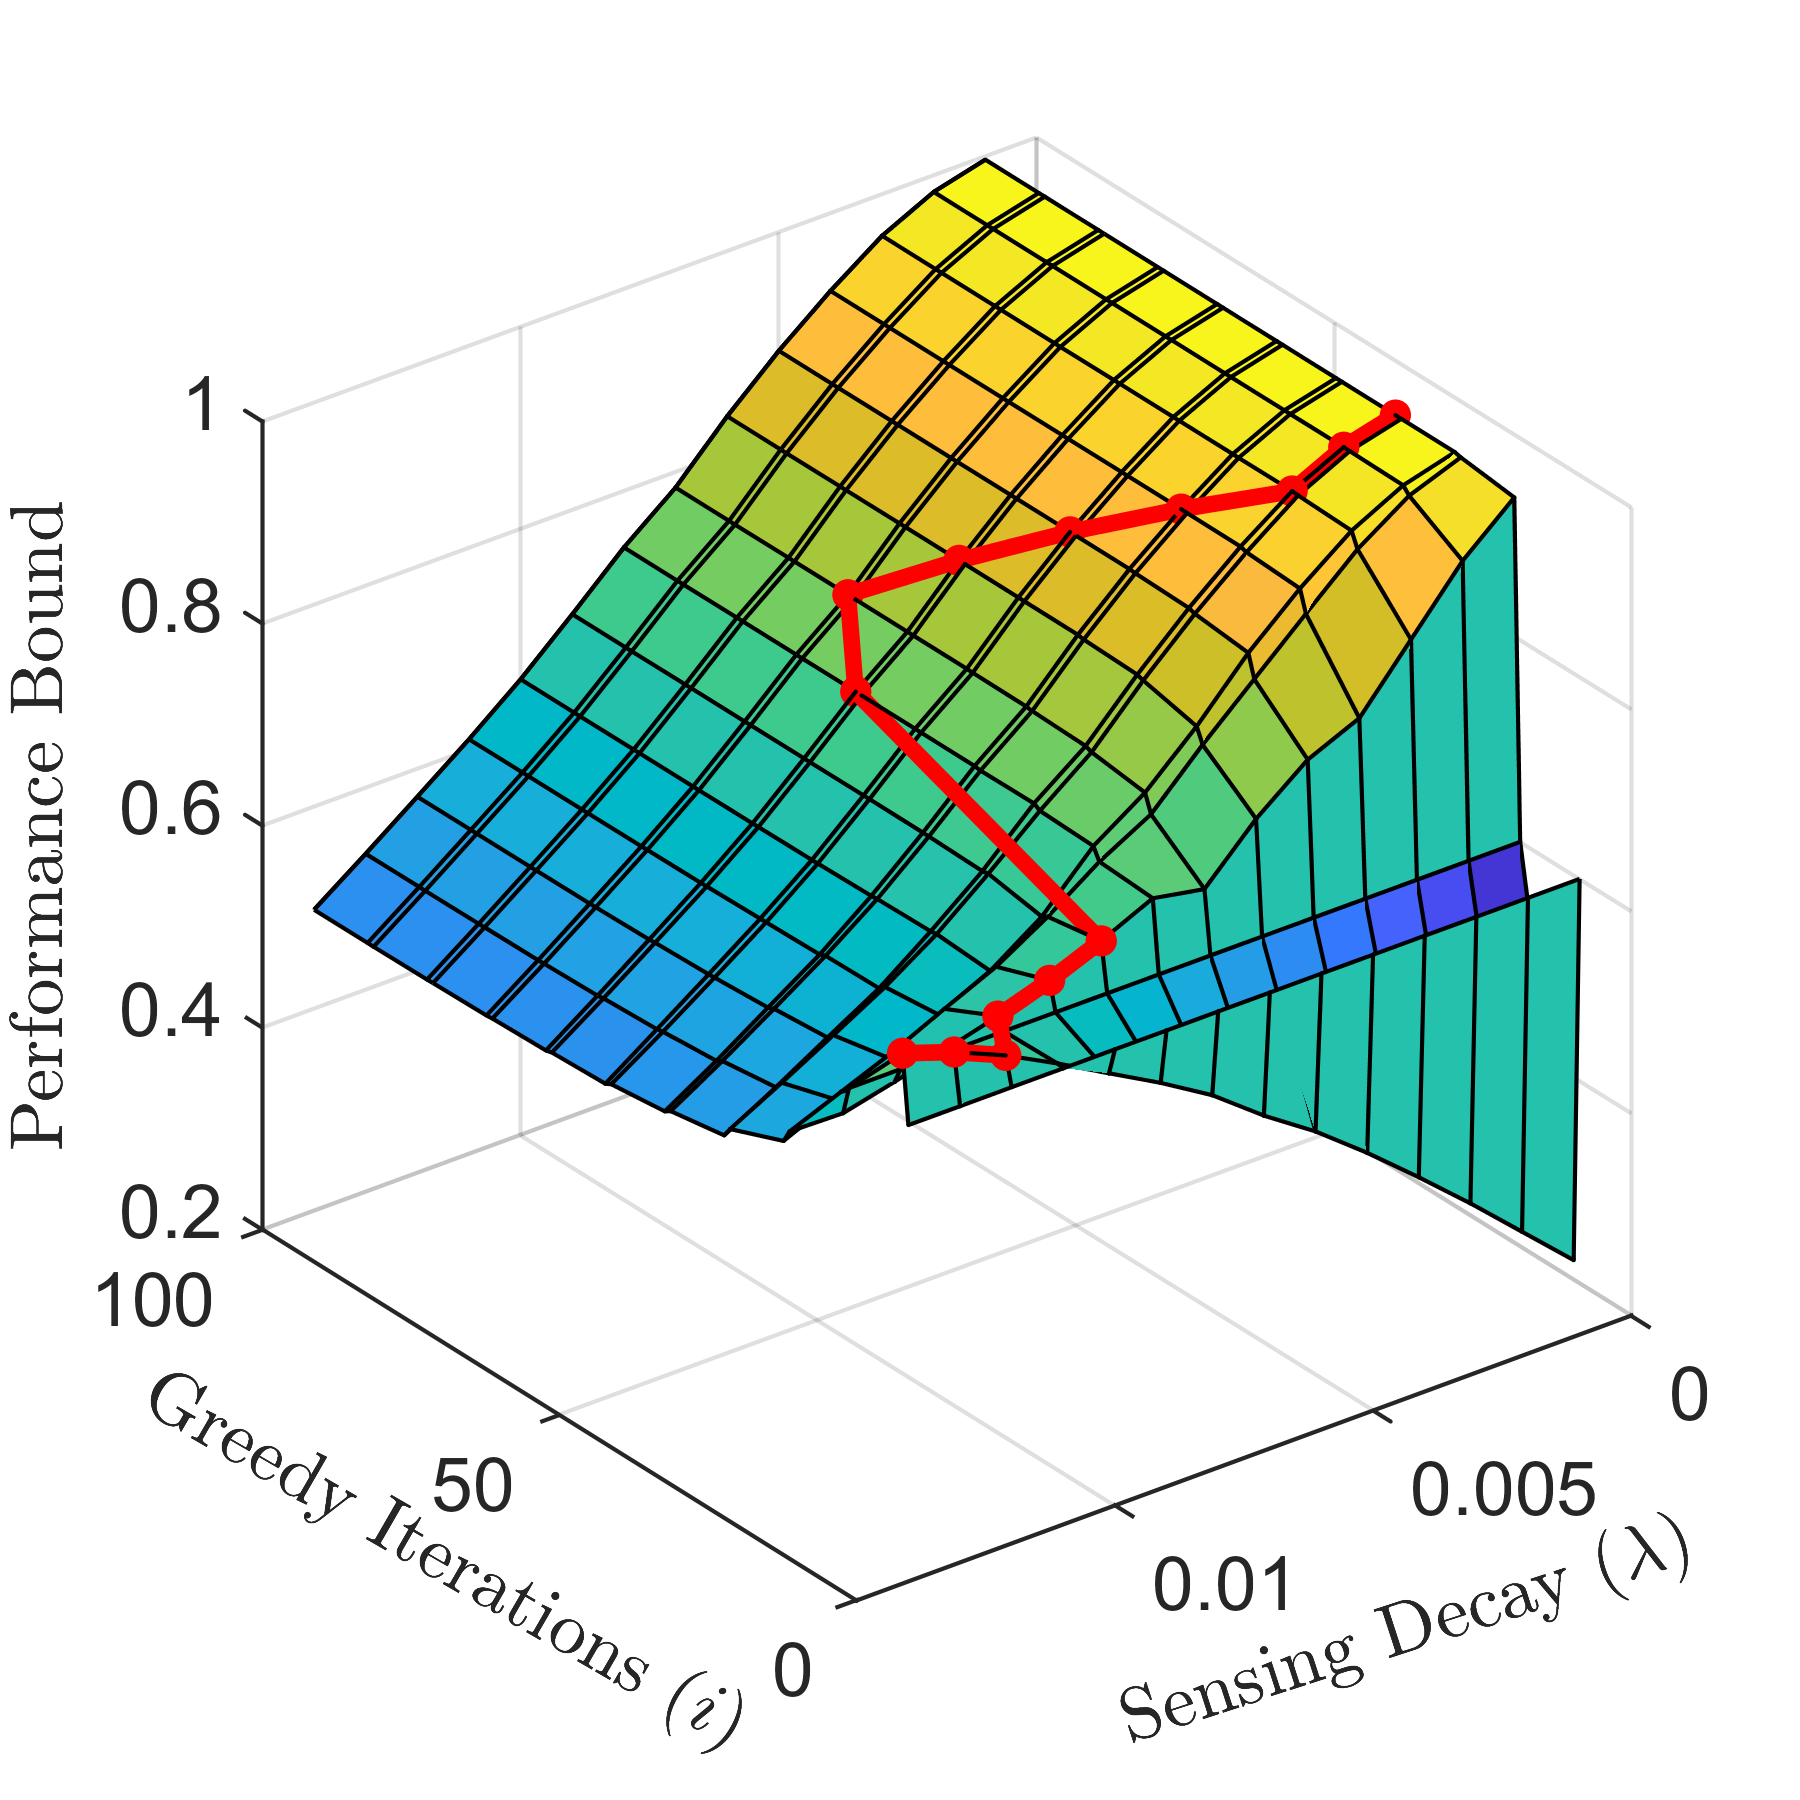
\includegraphics[width=2.5in]{Figures/Gen2_Exd1.png}
        \caption{The surface plot. Red line: $\beta_u$ vs. $\lambda$ vs. $i^*$.}
    \end{subfigure}%
    \\ \centering
    \begin{subfigure}[t]{0.17\textwidth}
        \centering
        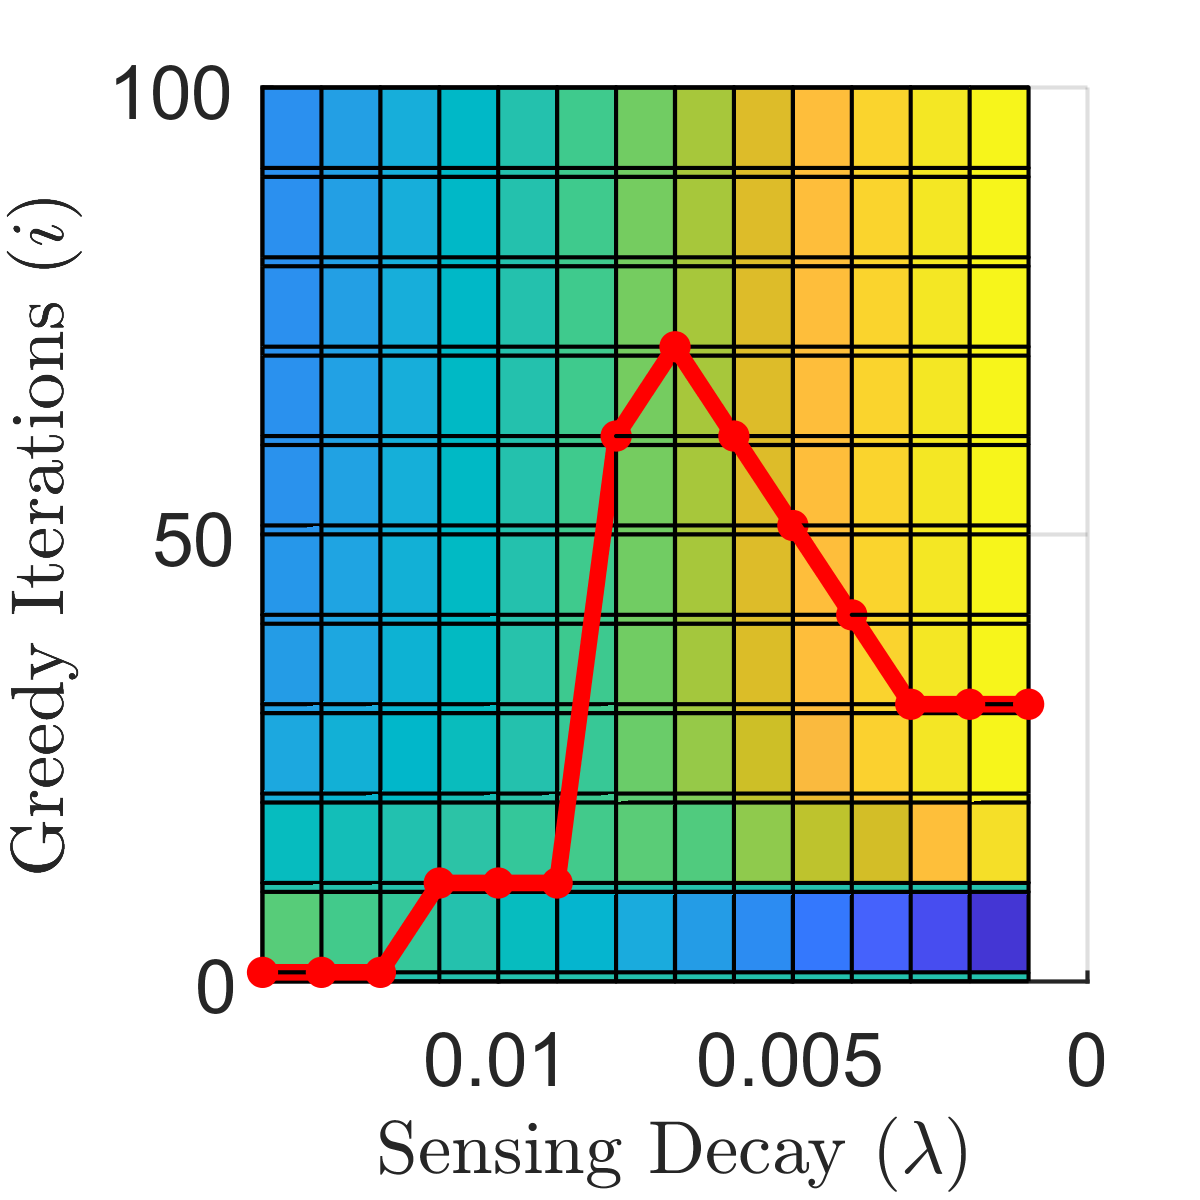
\includegraphics[width=\textwidth]{Figures/Gen2_Exd2.png}
        \caption{XY-View}
    \end{subfigure}
    \begin{subfigure}[t]{0.17\textwidth}
        \centering
        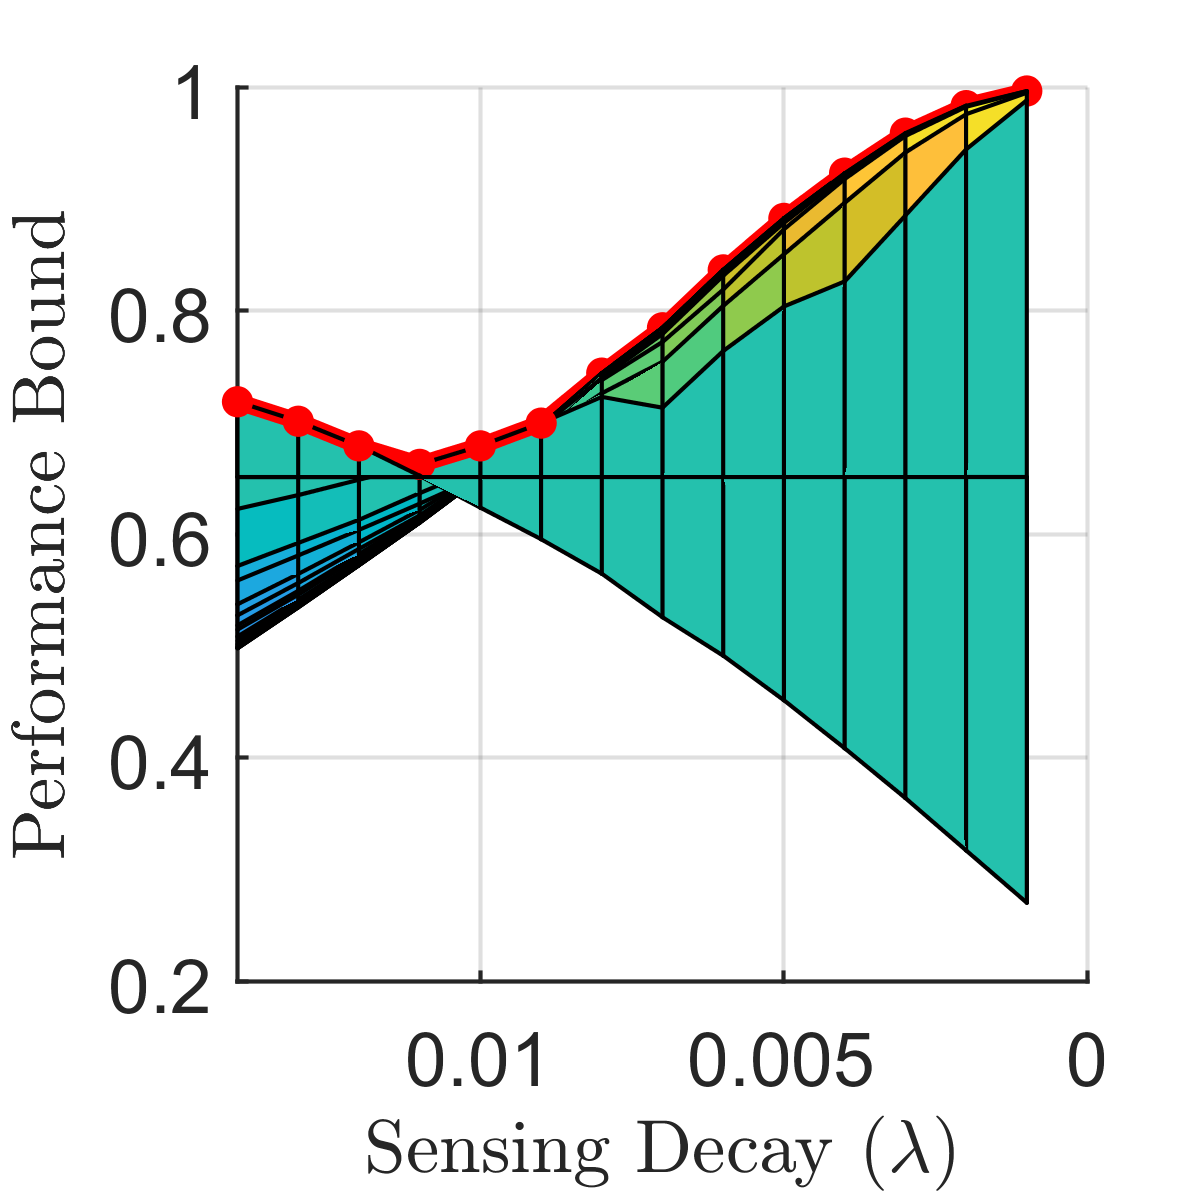
\includegraphics[width=\textwidth]{Figures/Gen2_Exd3.png}
        \caption{XZ-View (Fig. \ref{Fig:GeneralConfigBetaVsDecay}(a))}
    \end{subfigure}
    \caption{Extend Greedy Curvature Based Performance Bound vs. Sensing Decay Rate ($\lambda$) vs. No. of Greedy Iterations for the General mission space configuration with $\delta=400$, $N=10$.}
    \label{Fig:GeneralConfigBetaVsDecayVsiStar}
\end{figure}
 


\paragraph*{\textbf{Comparison with the previous work in} \cite{Sun2019,Sun2020}}
For this class of multi-agent coverage problems, the work in \cite{Sun2019} first proposed to adopt the performance bounds $\beta_t$ \eqref{Eq:TotalCurvatureBoundTheory} and $\beta_e$ \eqref{Eq:ElementalCurvatureBoundTheory} (from \cite{Conforti1984} and \cite{Wang2016}, respectively). Then, the subsequent work in \cite{Sun2020} proposed to adopt the performance bounds $\beta_g$ \eqref{Eq:GreedyCurvatureBoundTheory} and $\beta_p$ \eqref{Eq:PartialCurvatureBoundTheory} (from \cite{Conforti1984} and \cite{Liu2018}, respectively). The numerical results shown in Fig. \ref{Fig:BlankConfigBetaVsDecay} justify these contributions of \cite{Sun2019} and \cite{Sun2020} as they have lead to improved performance bounds compared to $\beta_f$. However, even in this case (Fig. \ref{Fig:BlankConfigBetaVsDecay}), it is notable that the proposed novel performance bound in this paper $\beta_u$ \eqref{Eq:Th:MainTheorem} has achieved an average improvement of $0.1248$ compared to the state of the art (i.e., compared to  $\max\{\beta_f,\beta_t,\beta_e,\beta_g,\beta_p\}$).


% Hence, future research can be is directed at improving the greedy algorithm and the performance bounds to address such challenging scenarios arising in submodular maximization problems.






\section{Conclusion}
\label{Sec:Conclusion}

In this paper, we considered the class of monotone submodular set function maximization problems subject to cardinality constraints. Different curvature measures and corresponding performance bounds found in the literature were reviewed for this class of problems, outlining their strengths and weaknesses. In particular, computational complexity, technical requirements and inherent limitations were the main weaknesses observed. A novel curvature measure was proposed along with a corresponding performance bound that does not suffer from the limitations identified in its predecessors. We named this curvature measure as the \emph{extended greedy curvature} since it thrives on the information seen when executing additional greedy iterations. A well-known class of multi-agent coverage problems was used to examine the effectiveness of the proposed performance bound compared to the other performance bounds found in the literature. Ongoing research explores the effectiveness of this new performance bound on other applications and under different quantified strength levels of the submodularity property.

\section*{Acknowledgment}
We are immensely grateful to Prof. David A. Casta\~n\'on, Prof. Sean B. Andersson and Prof. Ioannis Ch. Paschalidis of Boston University, Brookline, MA, USA, for sharing their expertise, insights and comments on an earlier version of this manuscript.  






\bibliographystyle{plainurl}
\bibliography{References} 

\end{document}